\chapter{The Askaryan Radio Array's Five Station Analysis \label{chap:5sa_analysis}}

  After reducing our 10\% data to a predominantly thermal-like collection of events, we construct an analysis that separates potential signal from our background. 
  This is done by training a Linear Discriminant Analysis (LDA) algorithm on each station-configuration.
  The LDA determines the linear projection of the data that provides the best separation between signal and background relative to their statistical spread, discussed further in Section~\ref{sec:lda}.
  The distribution of LDA values for thermal-like events is modeled and passed, along with the model of surface-like events identified in Section~\ref{sec:zc_slc}, to an optimization algorithm that identifies the best LDA cut for each station-configuration in the context of each array-wide configuration and the best Zenith Cut for the 6 instruments. 
  The optimization is explained in Section~\ref{sec:optimization}.

  Once the LDA cut (discriminating signal from background) and the Zenith Cut (rejecting cosmic rays and unparameterized anthropogenic noise) are optimized based on the 10\% sample and simulated neutrino events, the analysis is applied to the 100\% dataset. 
  Post-unblinding, we assess the compatibility of the models built on the 10\% data which drove the optimized LDA Cut and Zenith Cut are compared with the now-unblinded 100\% data.
  Any events that survive all analysis cuts (cleaning and LDA) are then passed through an isolation condition that removes any events that occurred between 5 seconds and 5.8 hours of each other, as we don't expect to find multiple neutrino events in close succession, except events that observe multiple particles or cascades (muon and tau tracks of stochastic losses and a tau decay), like those quantified in Fig.~\ref{fig:secondaries_contribution}. 
  We outline a plan for how to assess any remaining (``passing'') events, in case they are due to unforeseen backgrounds not present in the 10\% sample. 
  Lastly, we use the expected background rates and the number of passing events to establish an upper limit on the flux of UHE neutrinos. 

\section{The Linear Discriminant Analysis \label{sec:lda}}

  In this analysis, thermal background discrimination from expected neutrino signal is performed using a Linear Discriminant Analysis (LDA).
  Previous analyses have used the Fisher Discriminant~\citep{fisherDiscriminant, ara_pa_analysis} or a cut in the 2 dimensional distribution of event correlation against signal strength~\citep{ara_a23}. 
  An LDA is a generalization of Fisher Discriminants and, if only using two variables, performs similarly to separating signal and background by drawing a line in the 2 dimensional histogram of event correlation versus signal strength. 
  LDAs, for each event, will take an array of analysis variables and combine them linearly into a single number by multiplying the variables for each event against a matrix that's been optimized to minimize LDA scores for background events and maximize scores for signal events. 
  This analysis uses the 19 variables summarized in Table~\ref{tab:LDAvars} to train the LDA. 
  These 19 variables are chosen based on their ability to distinguish thermal-like events from neutrino events while minimizing correlations between the variables.
  This LDA is trained on a signal dataset composed of simulated neutrino events following the global experimental upper limit on the cosmic neutrino set (defined by Ref.~\citep{icecube_search-ehe} and Ref.~\citep{anita_iv}), and a background dataset composed of all events from each station's cleaned 10\% sample.   
  
  \begin{table}
    \centering
    \resizebox{0.9\textwidth}{!}{ % Shrink the table since it overflows a bit
      \begin{tabular}{c | p{0.8\linewidth} }
        Variable Name & Definition \\
        \hline
        \texttt{global\_max\_corr} & Maximum correlation score between all waveforms \\
        \texttt{global\_max\_corr\_v} & Maximum correlation score between waveforms from VPol antennas\\
        \texttt{global\_max\_corr\_h} & Maximum correlation score between waveforms from HPol antennas\\
        \texttt{avg\_snr\_v} & Average SNR of signals from VPol antennas \\
        \texttt{avg\_snr\_h} & Average SNR of signals from HPol antennas \\
        \texttt{hilbert\_snr\_v} & Average Hilbert Enveloped SNR of signals from VPol antennas \\ 
        \texttt{corr\_snr\_v} & Average SNR of the correlation function between all pairs of VPol antennas \\
        \texttt{csw\_snr\_v} & Coherently Summed Signal to Noise Ratio  in VPol antennas \\
        \texttt{avg\_rpr\_v} & Average SNR of signal power in VPol antennas \\ % Get a better definition
        \texttt{csw\_rpr\_v} & SNR of the power in the CSW from signals in VPol antennas \\ % Get a better definition
        \texttt{impulsivity\_v} & Power consumption during period maximal power consumption in the CSW compared to the rest of the CSW \\
        \texttt{bImp\_v} & Y-intercept of the linear fit to the latter portion of the impulsivity curve\\
        \texttt{mImp\_v} & Slope of the linear fit to the latter portion of the impulsivity curve \\
        \texttt{rhoImp\_v} & R-value of the linear fit to the latter portion of the impulsivity curve\\
        \texttt{impLinChi2\_v} & Difference between the linear fit to the latter portion of the impulsivity curve and a perfectly non-impulsive curve with a slope of 1. \\
        \texttt{impErfA\_v} & $A$ term in the functional fit to the impulsivity curve given by Equation~\ref{eq:functionalimp} \\
        \texttt{impErfB\_v} & $B$ term in the functional fit to the impulsivity curve given by Equation~\ref{eq:functionalimp} \\
        \texttt{impErfLinChi2\_v} & $\chi^2$ of the functional fit to the impulsivity curve given by Equation~\ref{eq:functionalimp} \\
        \texttt{impSig\_v} & Significance of the functional impulsivity fit given by Equation~\ref{eq:functionalimp} compared to the linear fit via Wilk's Theorem \\
      \end{tabular}
    }
    \caption{
        Analysis Variables used in the Linear Discriminant analysis along with a short description. 
        Full definitions of each variable can be found in Appendix~\ref{app:5savariables}.
    }
    \label{tab:LDAvars}
  \end{table}

  \begin{figure}
      \centering
      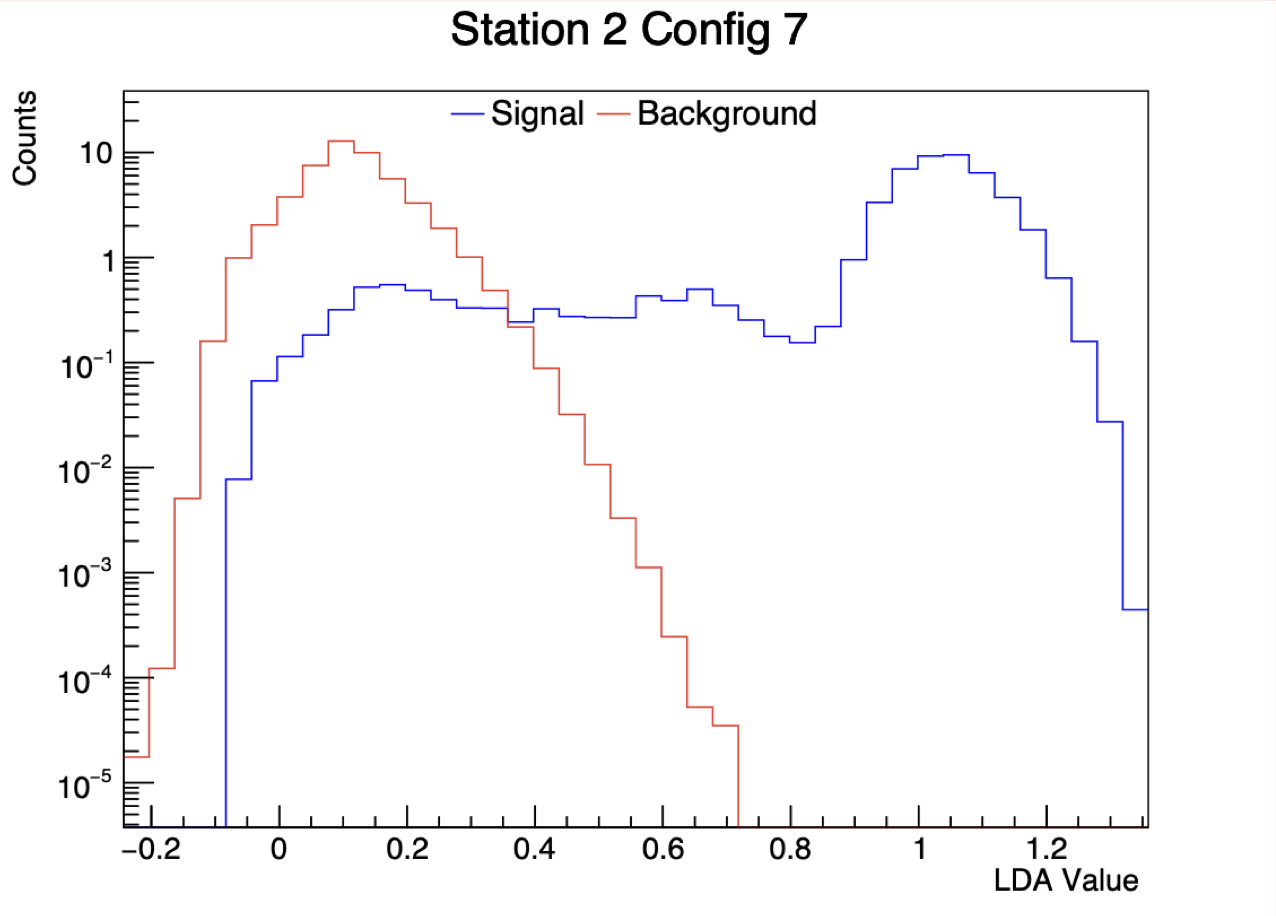
\includegraphics[
          width=0.75\textwidth,
          alt={}
      ]{sections/5sa-analysis/images/a2c7_lda_nudata.png}
      \caption{
        Distribution of Linear Discriminant Analysis scores for thermal-like background events (red, RF triggers that pass all cuts designed in Chapter~\ref{chap:5sa_cleaning}) from the 10\% sample and simulated neutrinos (blue) in A2 configuration 7.
      }
      \label{fig:ldafit}
  \end{figure}

  \begin{figure}
    \centering
    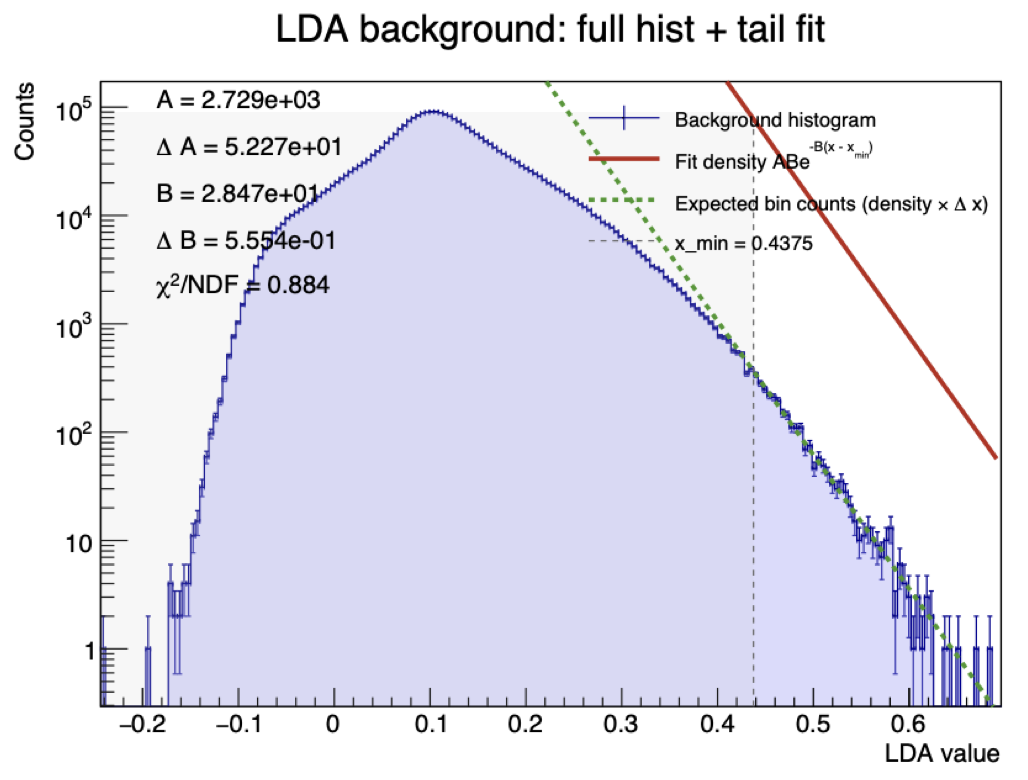
\includegraphics[
        width=0.75\textwidth,
        alt={}
    ]{sections/5sa-analysis/images/a2c7_10pct_lda_backgroundfit.png}
    \caption{
      Distribution of Linear Discriminant Analysis scores for the thermal-like background events (blue, RF triggers that pass all cuts designed in Chapter~\ref{chap:5sa_cleaning}) in the 10\% sample and from A2 configuration 7 fitted to an exponential (green).
      The fit is performed only on data $\geq x_{\text{min}}$.
      The fit is performed over a scan of $x_{\text{min}}$ values and the fit with the best reduced-$\chi^2$ is selected.
      The red curve shows the fit density (green line divided by the bin width, $\Delta x$).
    }
    \label{fig:backgroundfit_10pct}
  \end{figure}

  Once the LDA transformation matrix is optimized to separate thermal-like background events from neutrino events, we plot the LDA distributions for the signal and background datasets as show in Fig.~\ref{fig:ldafit}. 
  High statistics samples show that the tail of this distribution can be characterized by an exponential 
  \begin{equation}
    f(x) = A e^{-B (x-x_{\text{min}})}
    \label{eq:backgroundfit_exp}
  \end{equation}
  We fit the upper tail of the background event LDA distribution to this form and use it in the upcoming array-wide optimization. 
  In this context, $x$ is the central LDA value of the bin, $x_{\text{min}}$ is the LDA value above which the fitting is performed, and $A$ and $B$ are fit parameters. 
  An example of this fit is shown in Fig.~\ref{fig:backgroundfit_10pct} for the A2 configuration 7 thermal background LDA distribution. 

  We assess the integrity of the background tail fit via pseudoexperiments\index{Pseudoexperiment}.
  These pseudoexperiments use Poisson statistics to re-sample the LDA distribution shown in Fig.~\ref{fig:backgroundfit_10pct} according to a modified tail fit that has been subjected to Gaussian fluctuations.
  Variations in the model fit parameters characterize systematic uncertainties on the background model while re-sampling the LDA distribution characterizes statistical uncertainties. 
  Enumerated, this procedure is as follows: 
  \begin{enumerate}
    \item The parameters $A$ and $B$ in Eq.~\ref{eq:backgroundfit_exp} of the exponential tail model that was fit to real thermal background LDA values are re-sampled according to Gaussian fluctuations, obtaining a ``temporary" tail model. The fit error for $A$ and $B$ established when fitting the real thermal background model define the Gaussian widths for the fluctuations.
    \item For each bin in the LDA distribution, the temporary tail model is integrated over the bin to obtain a number of counts in the bin. This number of counts is then re-sampled following Poisson statistics.
    \item The log-likelihood of this re-sampled LDA distribution is calculated with respect to the original thermal background model.
    \item The above three steps are repeated 10,000 times and a distribution of log-likelihoods is plotted as shown in Fig.~\ref{fig:backgroundfit_10pct_toys}. The log-likelihood of the real observed distribution is also calculated with respect to the original thermal background model and plotted for reference. The fraction of toys with a log-likelihood greater than the observed log-likelihood (the p-value) is reported. 
  \end{enumerate}

  \begin{figure}
    \centering
    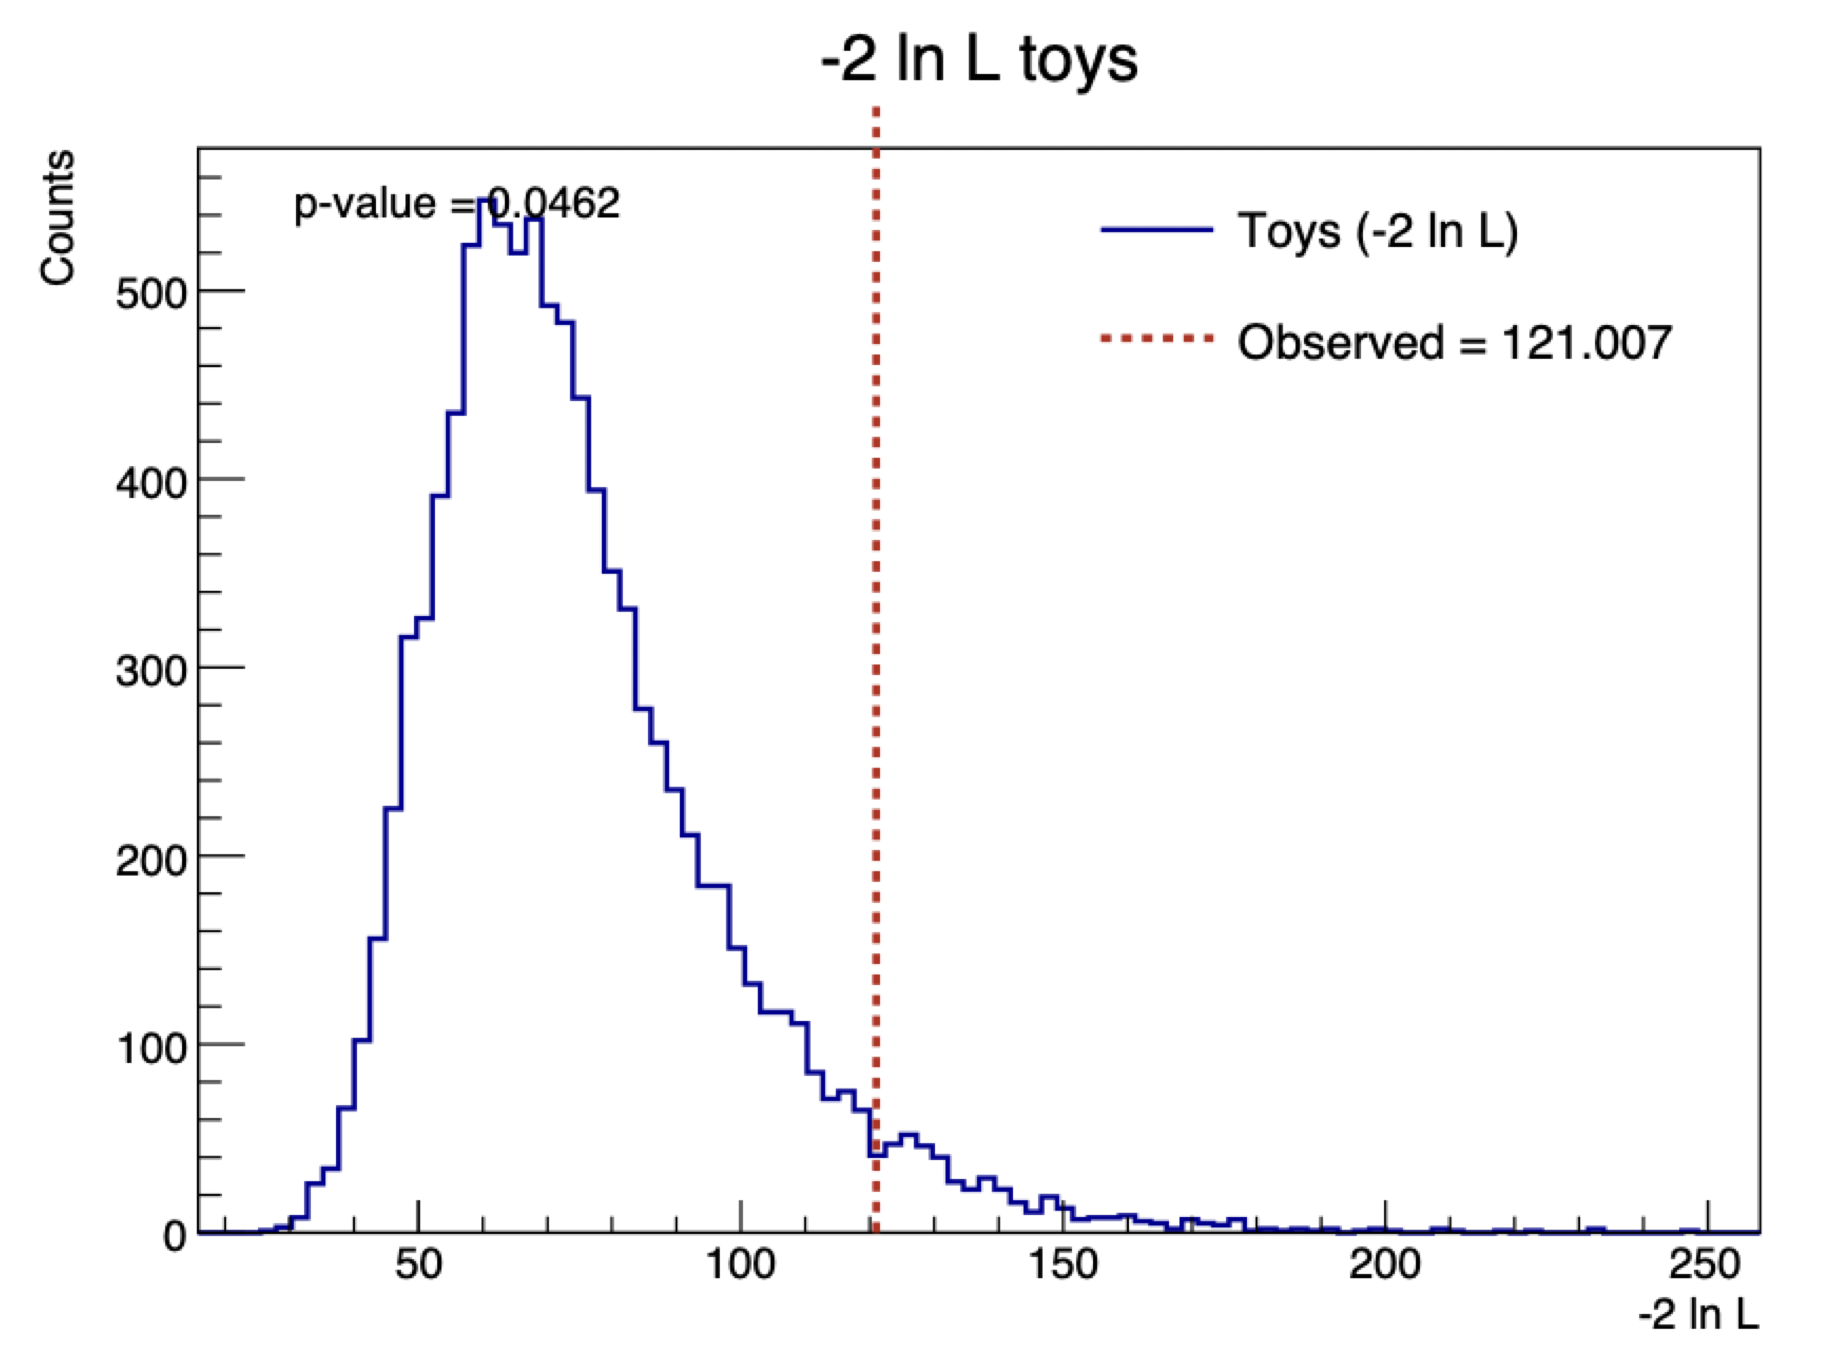
\includegraphics[
        width=0.75\textwidth,
        alt={}
    ]{sections/5sa-analysis/images/a2c7_100pct_lda_backgroundfit_toys.png}
    \caption{Distribution of log-likelihoods comparing background pseudoexperiments (blue) to the background model on observed 100\% A2 configuration 7 data (red).}
    \label{fig:backgroundfit_10pct_toys}
  \end{figure}

  At the end of this process, we have models of background LDA values for each station and configuration which will be combined for array-wide optimization.
  Note that as the LDA transformation matrix is optimized separately for each station-configuration, the resulting LDA scores for each station-configuration should not be compared to each other. 
  Said another way, if one station-configuration's LDA distribution ends at 1.2 and another ends at 1.4, this does not simply imply the former is better than the latter. 

\section{Optimization \label{sec:optimization}}

  After the thermal background LDA model determined in Section~\ref{sec:lda} and the surface event elevation models determined in Section~\ref{sec:zc_slc} for each station-configuration are set, we feed them both into an algorithm that determines the best LDA cut and Zenith Cut for each array-wide configuration. 
  An array-wide configuration is defined by the combination of active stations (in their respective station livetime configuration) over time periods of at least 1 week. 
  There are 50 total array-wide combinations of the 29 total station configurations, as shown in Fig.~\ref{fig:ARA_configurations}.
  Each LDA cut is established within each array-wide configuration. 
  For example, A2 configuration 7 is present in array-wide configurations 40, 42, 43, and 44 and has a different LDA cut optimized for each array-wide configuration in the parameter space of the same parent distribution.
  Expanding on this, across the full 50 array-wide configurations there are 144 LDA cuts to establish using the same 29 parent datasets. 
  We optimize just one zenith cut for each station (there are not enough statistics to do it based on station configuration like with the LDA).
  In total this results in 6 Zenith Cuts and 144 LDA Cuts to be optimized.
  The optimized A2 Zenith Cut is set to an elevation angle of $10.31^{\circ}$ and the minimum and maximum LDA cut for each A2 configuration are presented in Table~\ref{tab:ldacuts}. 
  The signal efficiency of the analysis over the entire array is plotted as a function of simulated neutrino energy in Fig.~\ref{fig:LDA_efficiency_wLDA} with the optimized LDA applied.

  \begin{table}
    \centering
    \begin{tabular}{cc}
      Livetime Configuration & LDA Cut Range \\
      \hline
      1 & 0.95 - 0.99 \\
      2 & 1.14 \\
      3 & 0.90 - 0.91 \\
      4 & 1.01 - 1.02 \\
      5 & 1.15 - 1.34 \\
      6 & 1.11 - 1.23 \\
      7 & 0.97 - 1.00 \\
    \end{tabular}
    \caption{
      Range of cuts used to distinguish thermal background events from neutrino signal events, after optimization. 
    }
    \label{tab:ldacuts}
  \end{table}

  \begin{figure}
    \centering
    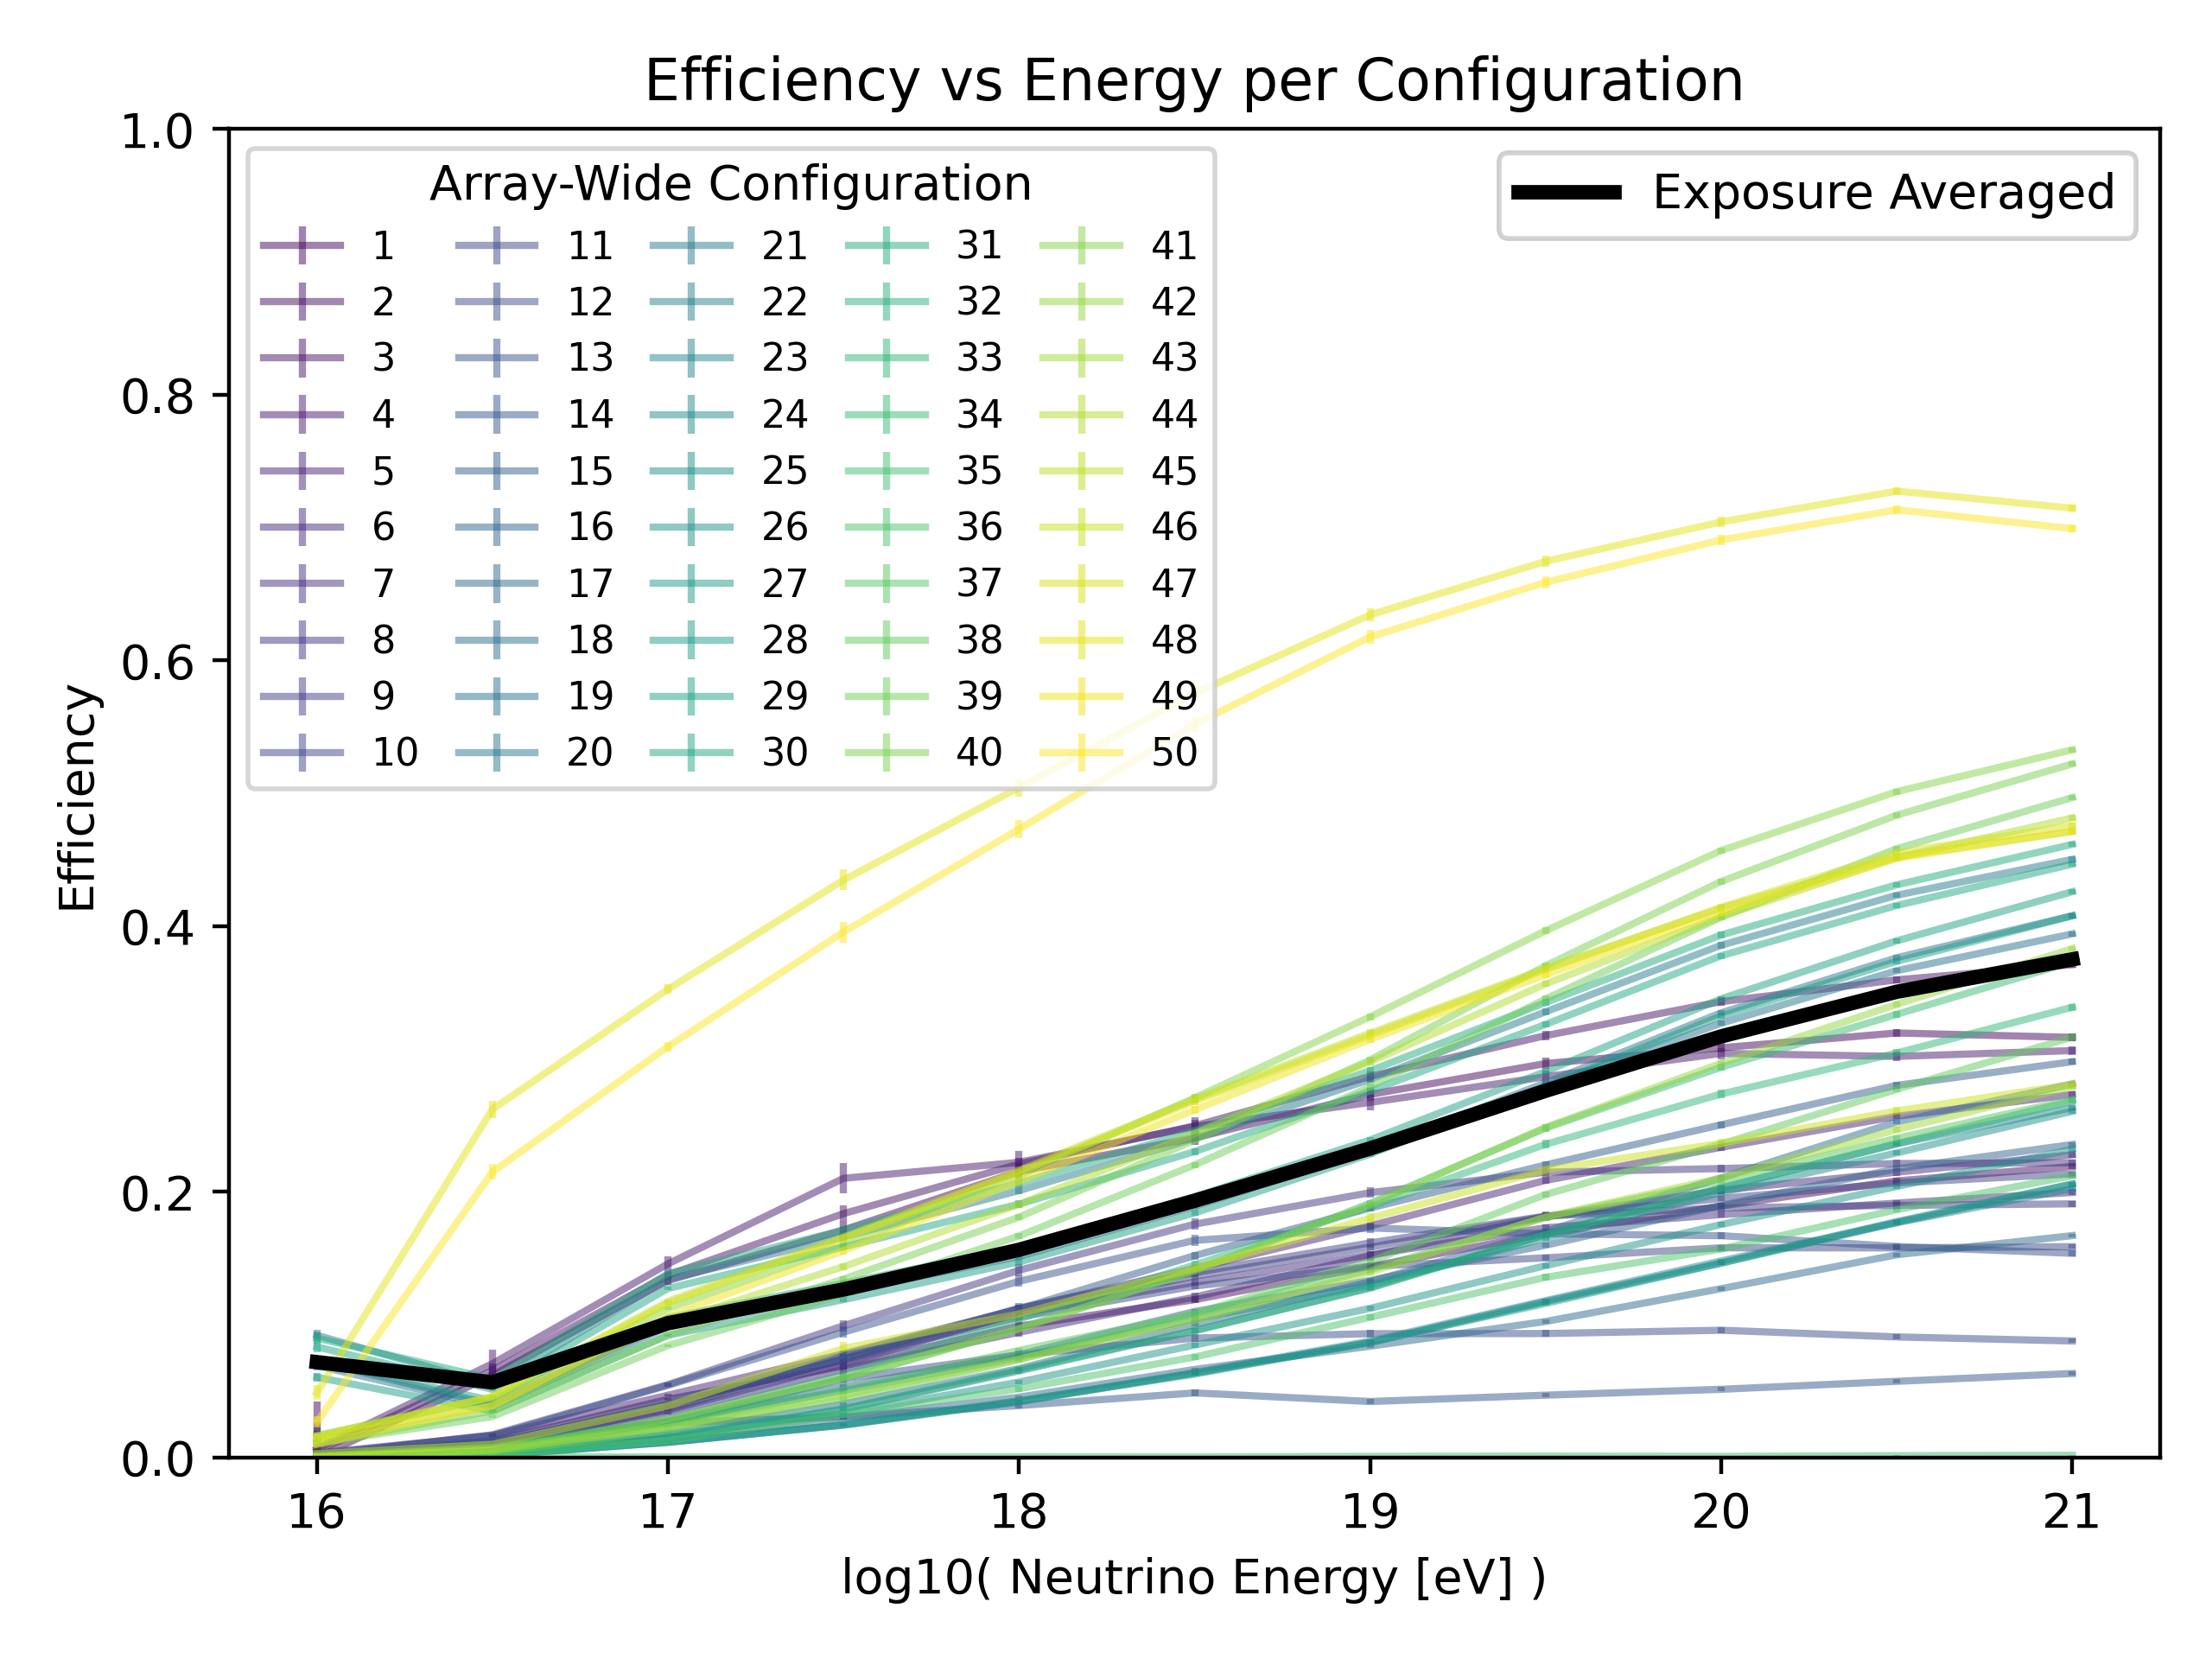
\includegraphics[
      width=0.7\linewidth,
      alt={}
    ]{sections/5sa-analysis/images/arraywide_efficiencies_vs_energy.png}
    \caption{
      Array-wide signal efficiency for each array-wide configuration (colored lines) and the exposure-weighted efficiency over all array-wide configurations (black lines) presented as a function of neutrino energy. 
      The two lines with the greatest signal efficiency are for array-wide configuration 48 and 50 during both of which, only the PA was active therefore demonstrating the signal efficiency of the PA detector in isolation.
      This represents the array-wide signal efficiency after all cleaning cuts defined in Chapter~\ref{chap:5sa_cleaning} were applied (using Zenith Cuts and Surface Like Cuts optimized in this section) and after the optimized LDA cut was applied.
    }
    \label{fig:LDA_efficiency_wLDA}
  \end{figure}

\section{Post-Unblinding Analysis \label{sec:unblinding}}

  Running the analysis pipeline over the full 100\% data and viewing which events survived all cuts for the first time is commonly referred to as ``opening the box". 
  After opening the box we investigate any events that pass the analysis and construct our analysis' sensitivity to UHE neutrinos.
  But, before we analyze the full data sample, we ensure that the surface background elevation model and the thermal background LDA model constructed with the 10\% dataset and used to establish the final Zenith and LDA Cuts are compatible with the 100\% data. 
  There is also one final cut to remove any array-wide temporal clusters of events which removes events that occur array-wide called the Time Isolation Cut.

  \subsection{Surface Cut Cross Checks}

    \begin{figure}
      \centering
      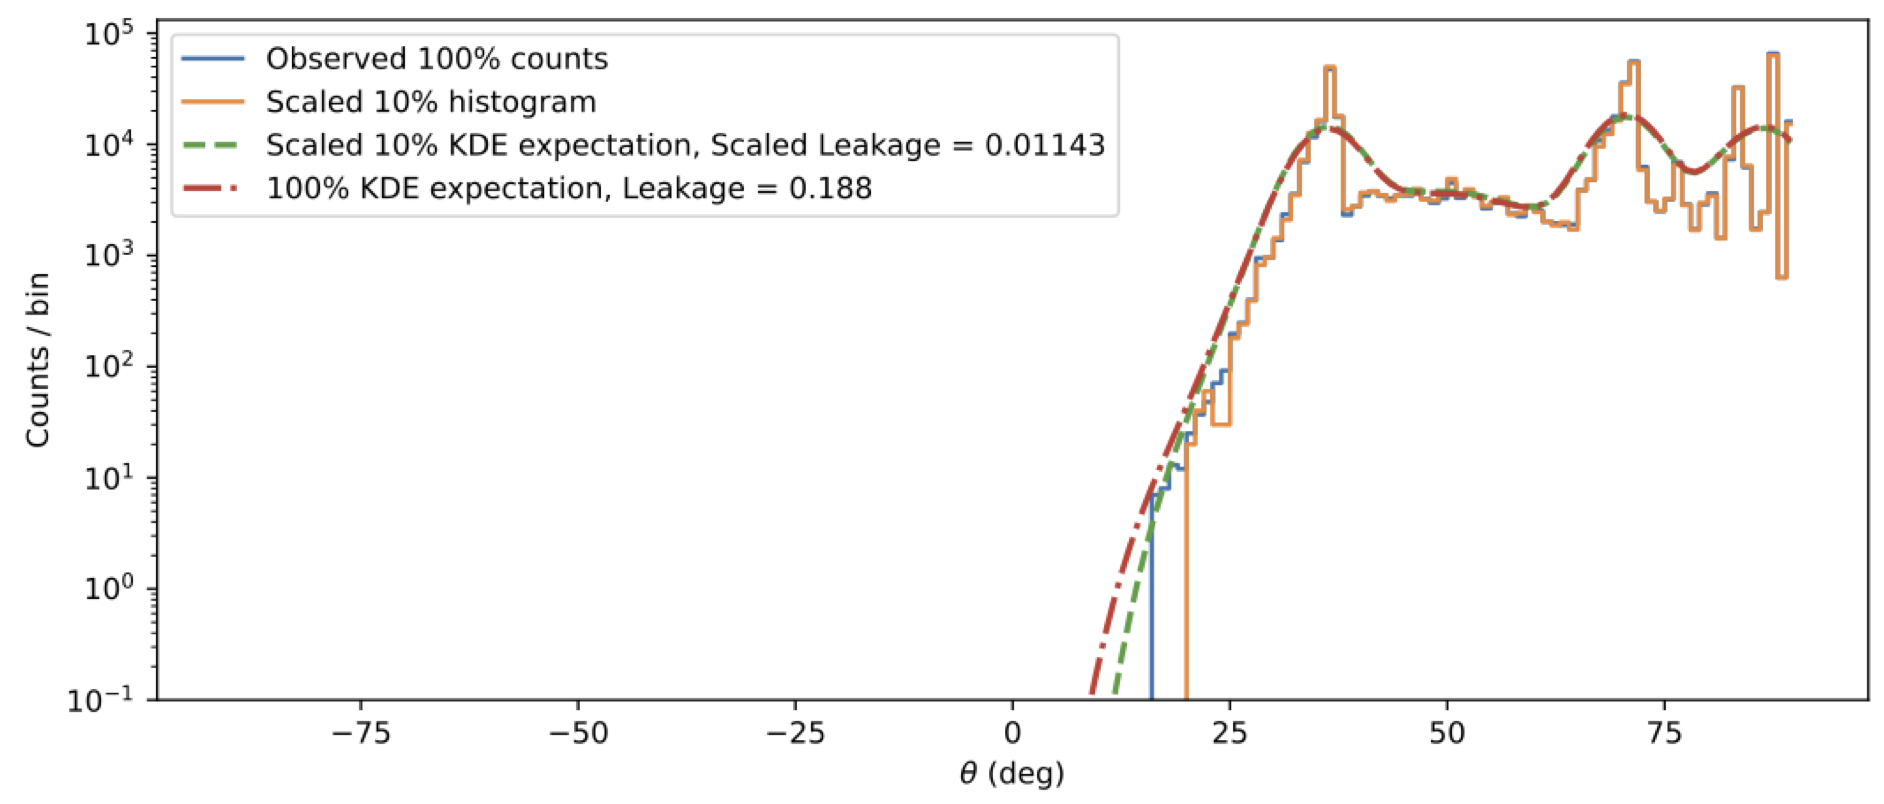
\includegraphics[
          width=\textwidth,
          alt={}
      ]{sections/5sa-analysis/images/a2_100pct_surfacecheck_zenithdist.png}
      \caption{
        The A2 surface background dataset built with the 10\% data and multiplied by 10 (orange) is compared to the surface background dataset built with the 100\% data (blue), as described in Section~\ref{sec:zc_slc}.
        The background model built on the 10\% dataset multiplied by 10 (green) compared to a model built on the 100\% dataset (red).
        The number of events that pass this cut is calculated as the number of events calculated using the red 100\% KDE line with an elevation angle below the optimized Zenith Cut of $10.31^{\circ}$.
      }
      \label{fig:backgroundcheck_zenith_dist}
    \end{figure}

    The first post-unblinding check is to build a surface event dataset and model (as described in Section~\ref{sec:zc_slc}) using the 100\% datasets then compare it to the model built with the 10\% data. 
    The distribution of event elevations in the surface dataset built with 100\% data is shown in Fig.~\ref{fig:backgroundcheck_zenith_dist} which shows strong visual agreement between the model built on the 10\% and the 100\% datasets. 
    All events in the 100\% distribution that have an elevation less than the lowest bin edge from the 10\% distribution have a \texttt{mindepth\_v} score greater than -5~m.
    This means that each event's highest reconstructed source origin (within 300~m) with a reconstruction correlation score at least 60\% of the all-sky maximum is at least -5~m. 
    Events originating from the surface have similar \texttt{mindepth\_v} scores.

    % \begin{figure}
    %   \centering
    %   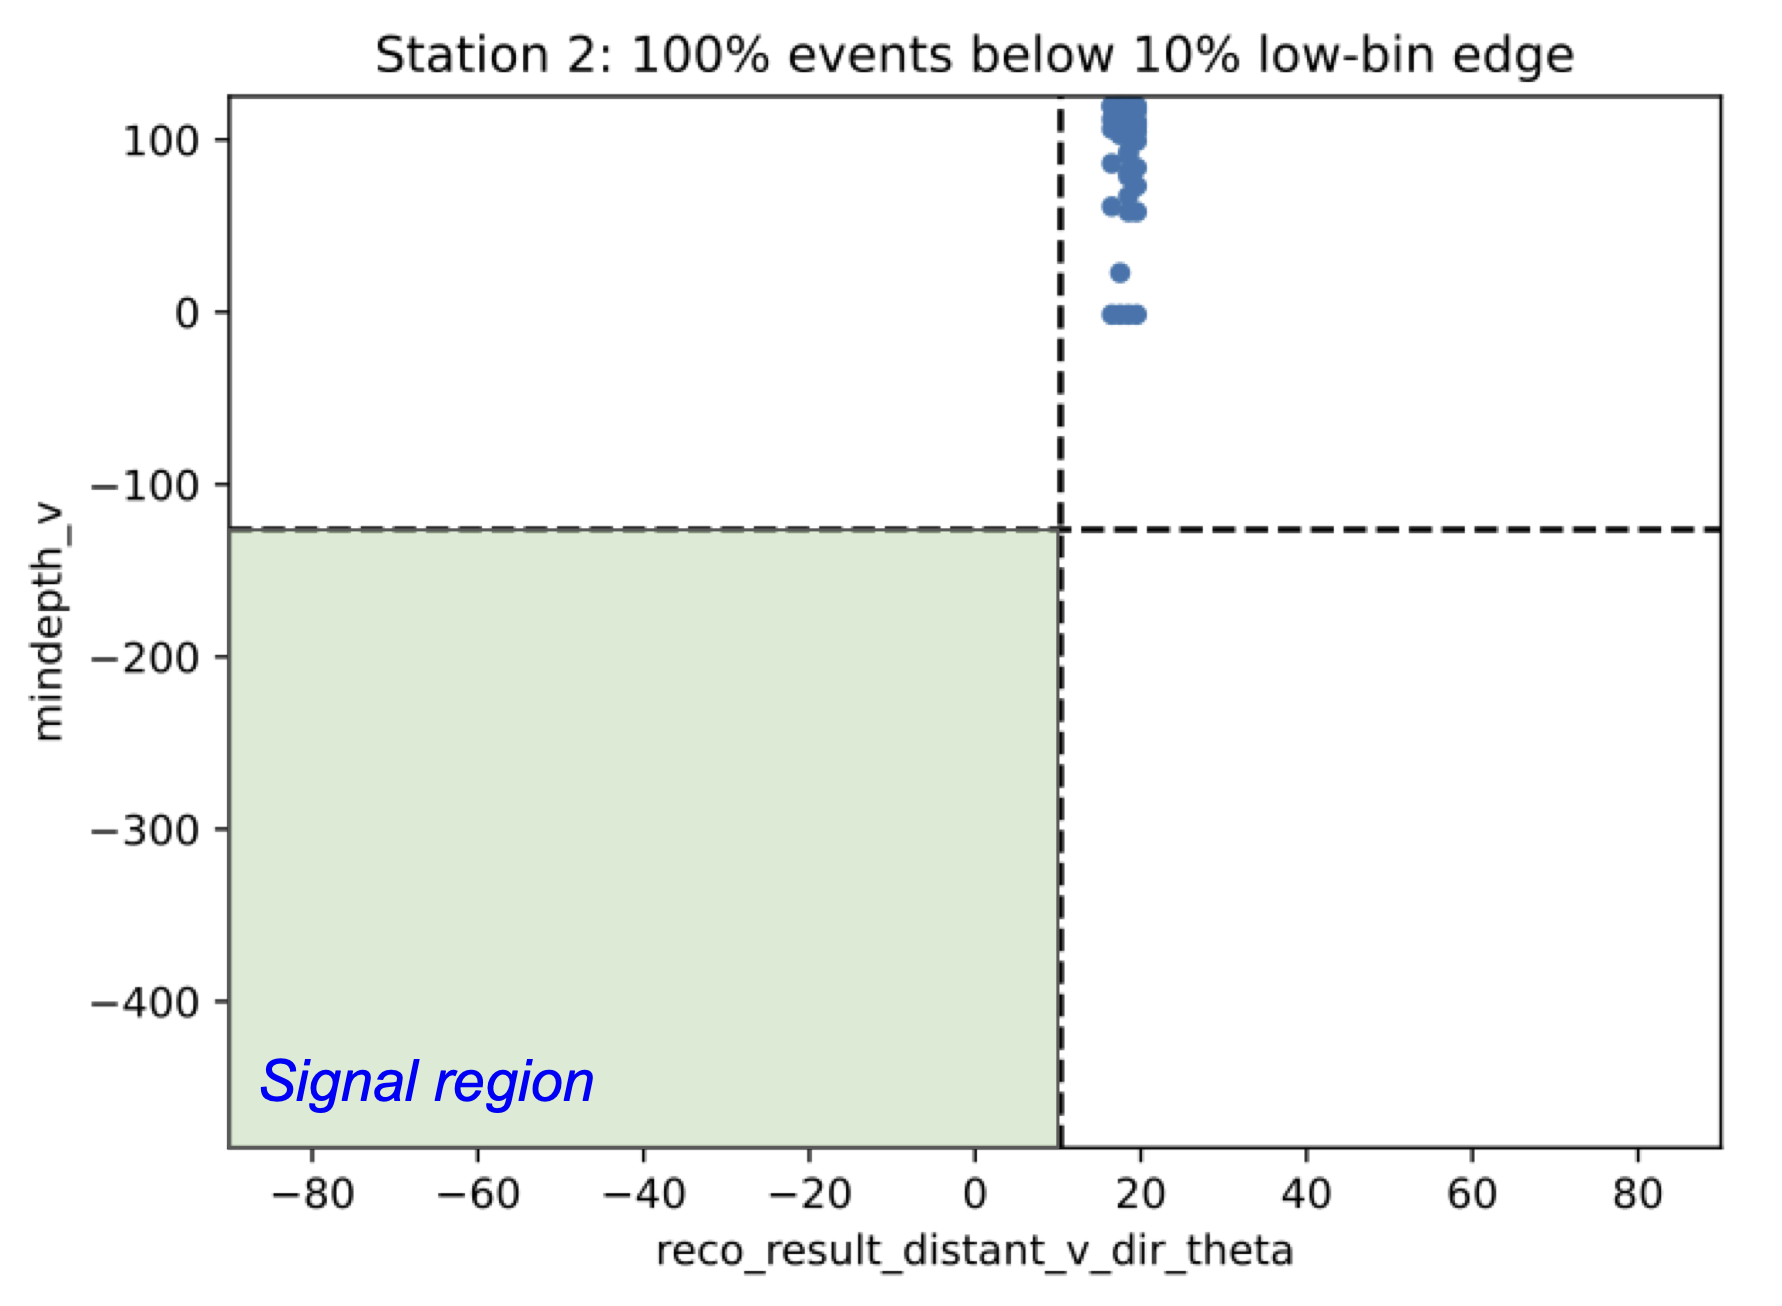
\includegraphics[
    %       width=0.75\textwidth,
    %       alt={}
    %   ]{sections/5sa-analysis/images/a2_100pct_surfacecheck_outliers.png}
    %   \caption{
    %     Distribution of events from the full 100\% dataset with reconstructed elevations less than the lowest bin in the 10\% dataset (as shown in Fig.~\ref{fig:backgroundcheck_zenith_dist}) plotted by their reconstructed elevation and \texttt{mindepth\_v}.
    %     As these events all have a \texttt{mindepth\_v} value sufficiently above the \texttt{mindepth\_v} cut established by the Zenith Cut optimization, these outliers do not suggest we have not modeled our surface background too loosely.
    %   }
    %   \label{fig:backgroundcheck_zenith_outliers}
    % \end{figure}

    % The 2 dimensional distribution of \texttt{mindepth\_v}\index{\texttt{L2 Variable: mindepth\_v}} and reconstructed elevations for events in the 100\% dataset that reconstruct below $20^{\circ}$, the lowest bin in the 10\% dataset, is shown in Fig.~\ref{fig:backgroundcheck_zenith_outliers}. 
    % The \texttt{mindepth\_v} parameter describes the minimum depth (converted from elevation angle) where the correlation score of an event's reconstruction is at least 60\% of the full reconstruction's maximum correlation score. 
    % Higher values of \texttt{mindepth\_v} indicate higher probabilities that an event originated from near and above the surface of the ice, where our data sample is largely contaminated by anthropogenic backgrounds and cosmic ray events.
    % This plot was created to ensure that none of these events in the 100\% surface data set with a reconstructed elevation less than $20^{\circ}$ were likely to have originated in the ice where we are searching for neutrinos. 
    % Figure~\ref{fig:backgroundcheck_zenith_outliers} shows that all of these events had a \texttt{mindepth\_v} of at least -1.7~m - meaning these events all had a high probability of originating near or above the surface and do not invalidate our background model.

    \begin{figure}
      \centering
      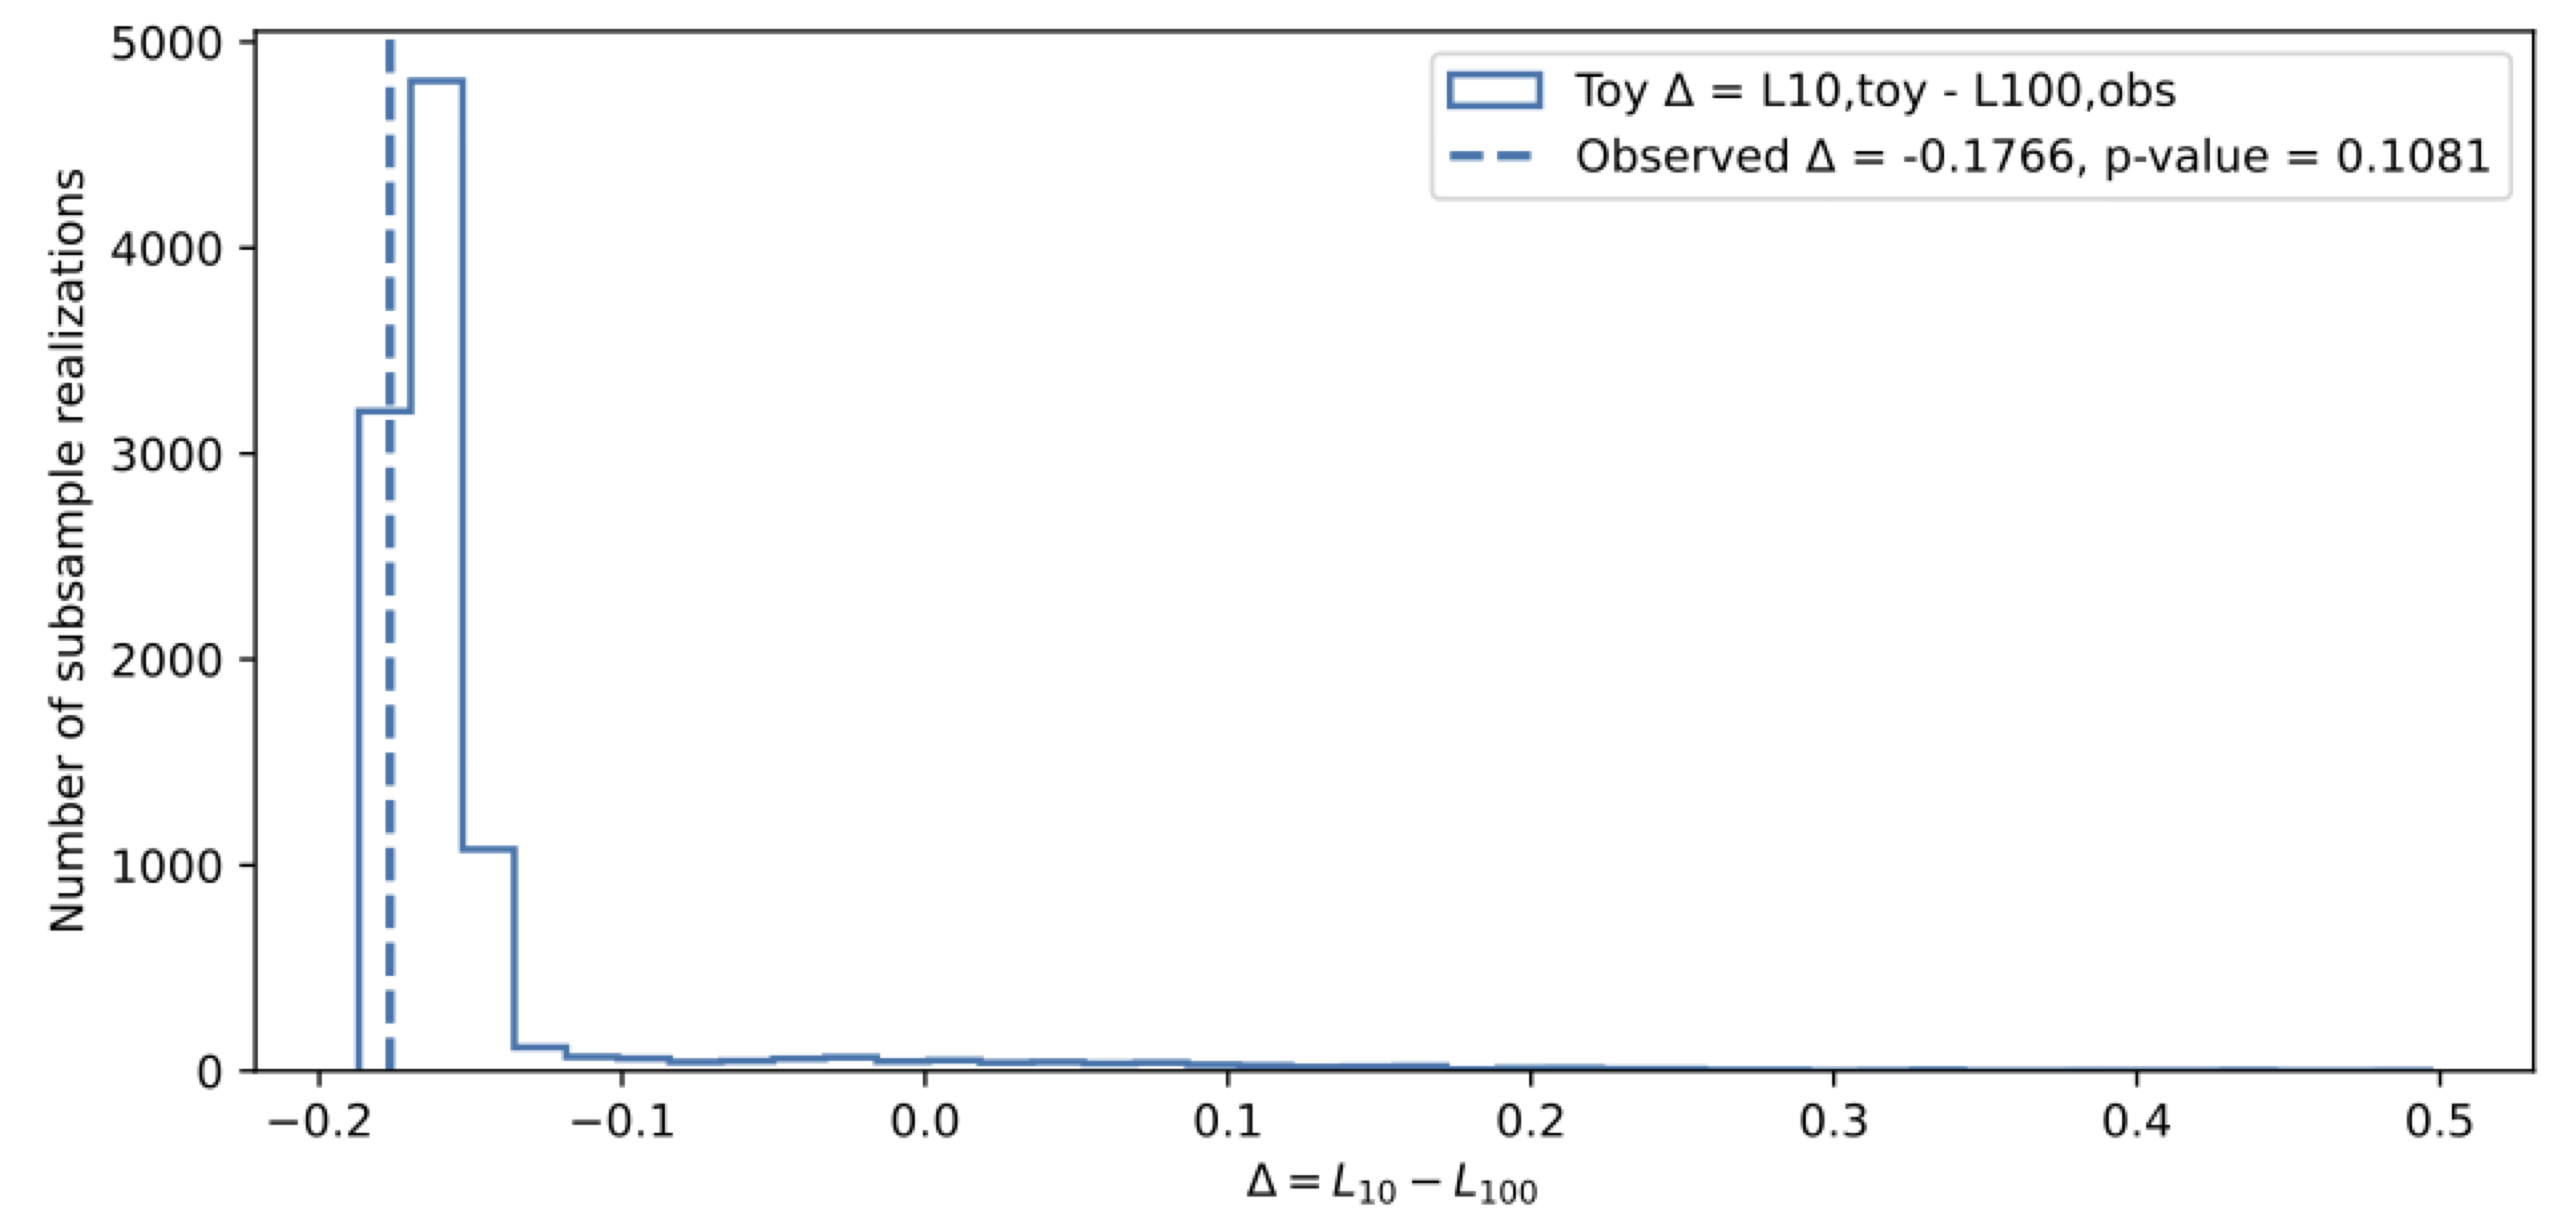
\includegraphics[
          width=\textwidth,
          alt={}
      ]{sections/5sa-analysis/images/a2_100pct_surfacecheck_toys.png}
      \caption{
        Distribution of the difference between surface background pseudoexperiments' log likelihood calculated against the model built on the 10\% and 100\% datasets (solid histogram). 
        The difference between the log likelihood of the 10\% and 100\% model compared to the observed 100\% surface background event distribution is plotted for comparison (dashed line).
      }
      \label{fig:backgroundcheck_zenith_toys}
    \end{figure}

    To quantify the agreement between the background model predicted by the 10\% sample and the one observed in the 100\% sample, we ran pseudoexperiments following a similar procedure used in Section~\ref{sec:optimization}. 
    The distribution of pseudoexperiments in relation to the observed log-likelihood with respect to the surface background model is shown in Fig.\ref{fig:backgroundcheck_zenith_toys}.
    The A2 model built on the 10\% data passed our check as the p-vale of the observed log-likelihood compared to the pseudoexperiments was greater than 0.05.
    The models for all other stations also passed this check. 

  \subsection{Thermal Background Cross Checks}

    Verifying the thermal background LDA model is performed similarly to the surface background elevation model. 
    We ensure that the thermal distribution of LDA values in the 100\% dataset is comparable to the fit made with 10\% sample via pseudoexperiments. 
    First, we plot the distribution of LDA values for thermal-like events in the 100\% data with LDA scores below the LDA cut value established in the optimization procedure defined in Section~\ref{sec:optimization}, as shown in Fig.~\ref{fig:backgroundcheck_a2c3} and Fig.~\ref{fig:backgroundcheck_a2c4} for configurations 3 and 4 of A2, respectively. 
    The pseudoexperiments are run next and if the observed log-likelihood is an outlier compared to the pseudoexperiments then the background model is assessed.
    This happened for both configurations 3 and 4 of A2 as shown in Fig.~\ref{fig:backgroundcheck_a2c3_toys} and Fig.~\ref{fig:backgroundcheck_a2c4_toys}, respectively.
    % How did we pick the outliers that we showed? 
    Results for the other stations are not discussed in this thesis but many configurations passed this thermal background check and those that did not were resolved in a similar fashion.

    \begin{figure}
      \centering
      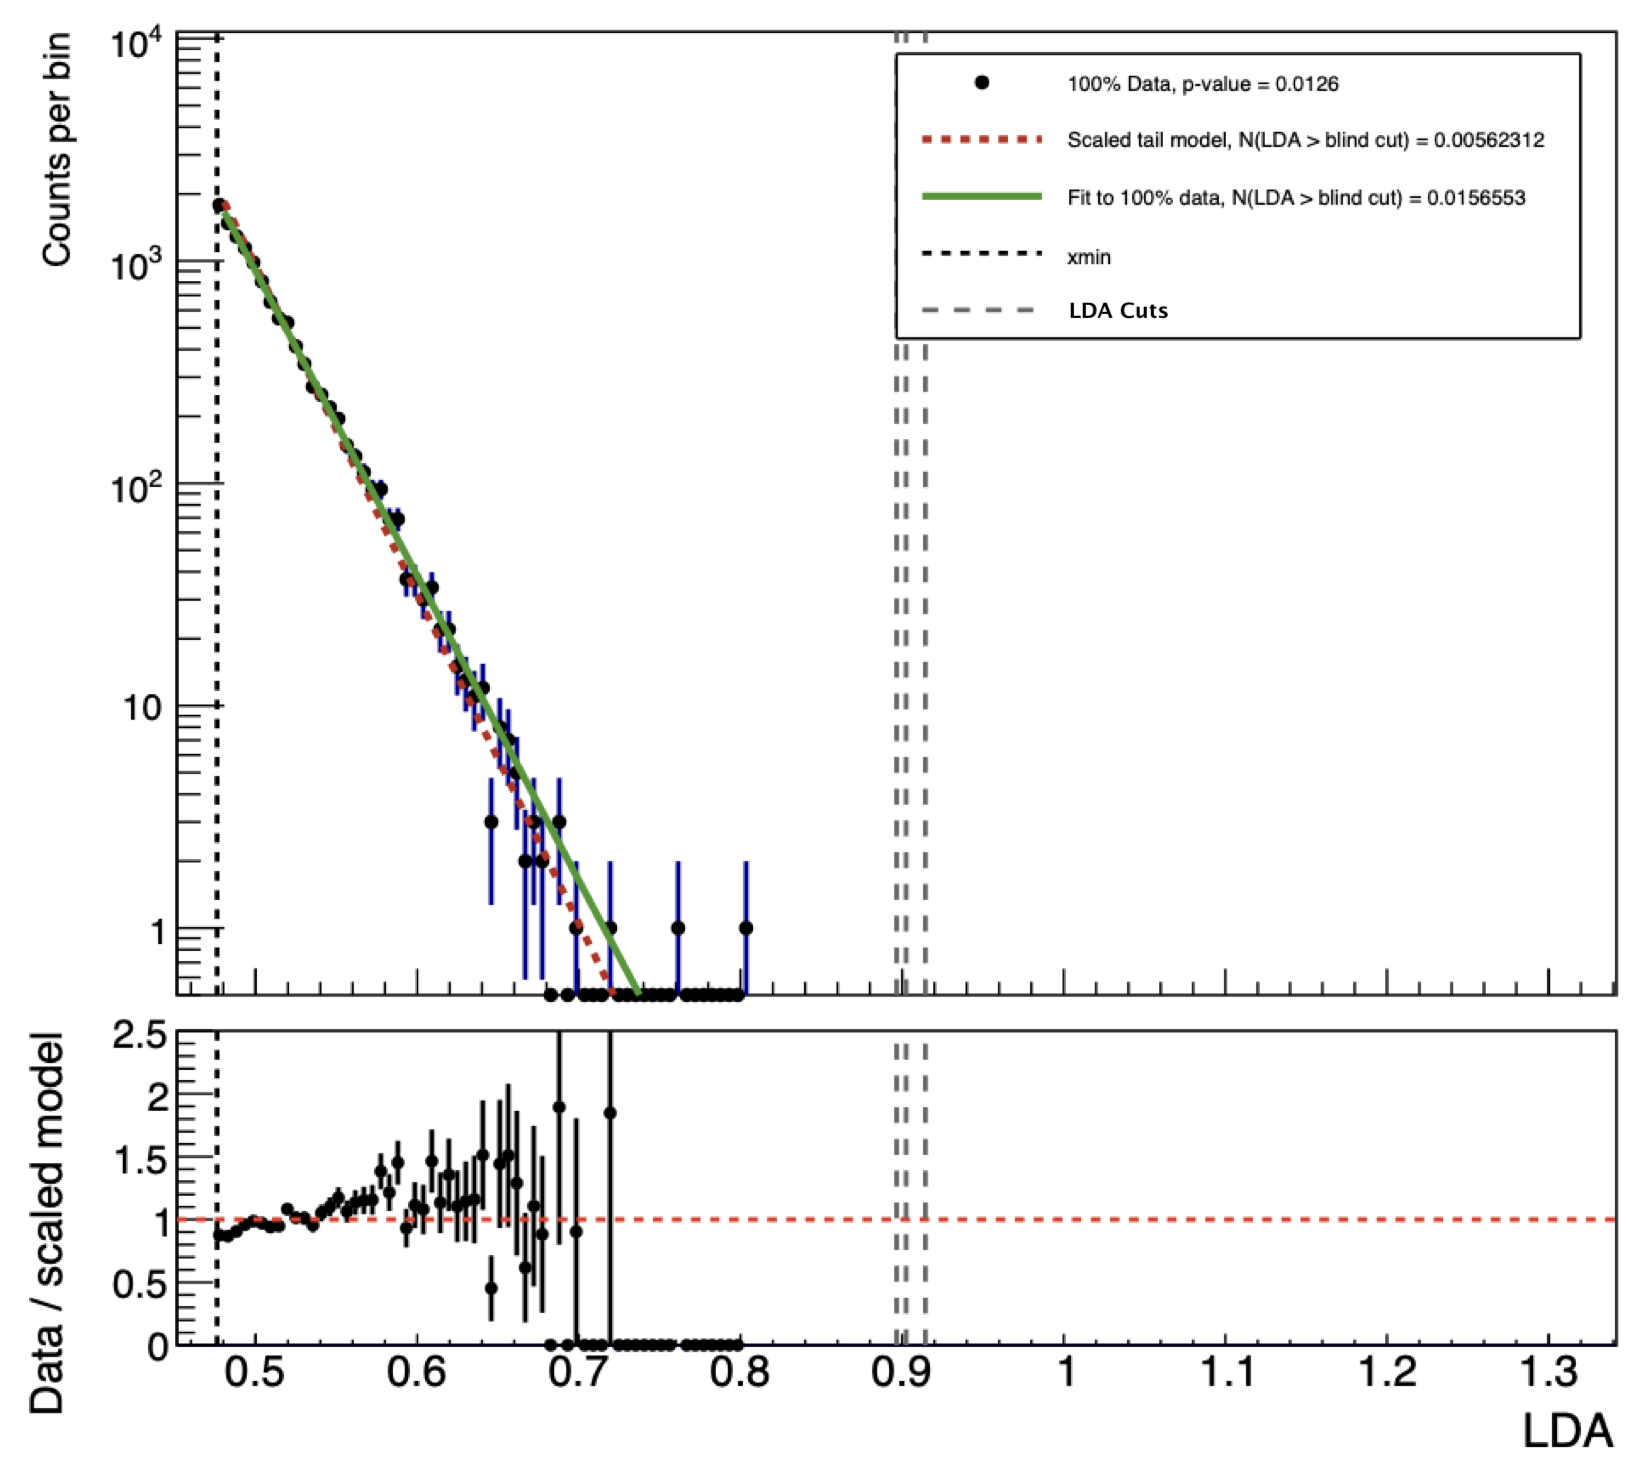
\includegraphics[
          width=0.75\textwidth,
          alt={}
      ]{sections/5sa-analysis/images/a2c3_100pct_lda_backgroundfit.png}
      \caption{
        Top: The distribution of thermal events (events that passed all cuts defined in Chapter~\ref{chap:5sa_cleaning}) from the 100\% sample of A2 configuration 3 (black dots with blue error bars).
        Only events with LDA scores greater than the $x_{\text{min}}$ used to fit the background model in Section~\ref{sec:lda} (black dotted line) and less than the appropriate LDA Cut established in Section~\ref{sec:optimization} are plotted (grey dashed lines).
        These are events are fit to an exponential (green line) plotted along the model built on the 10\% data multiplied by 10 (red dotted line).
        Bottom: Ratio of the 100\% LDA distribution of thermal events (black dots in top panel) divided by the model built on the 10\% data scaled up by a factor of 10 (red dotted line in top panel).
      }
      \label{fig:backgroundcheck_a2c3}
    \end{figure}

    \begin{figure}
      \centering
      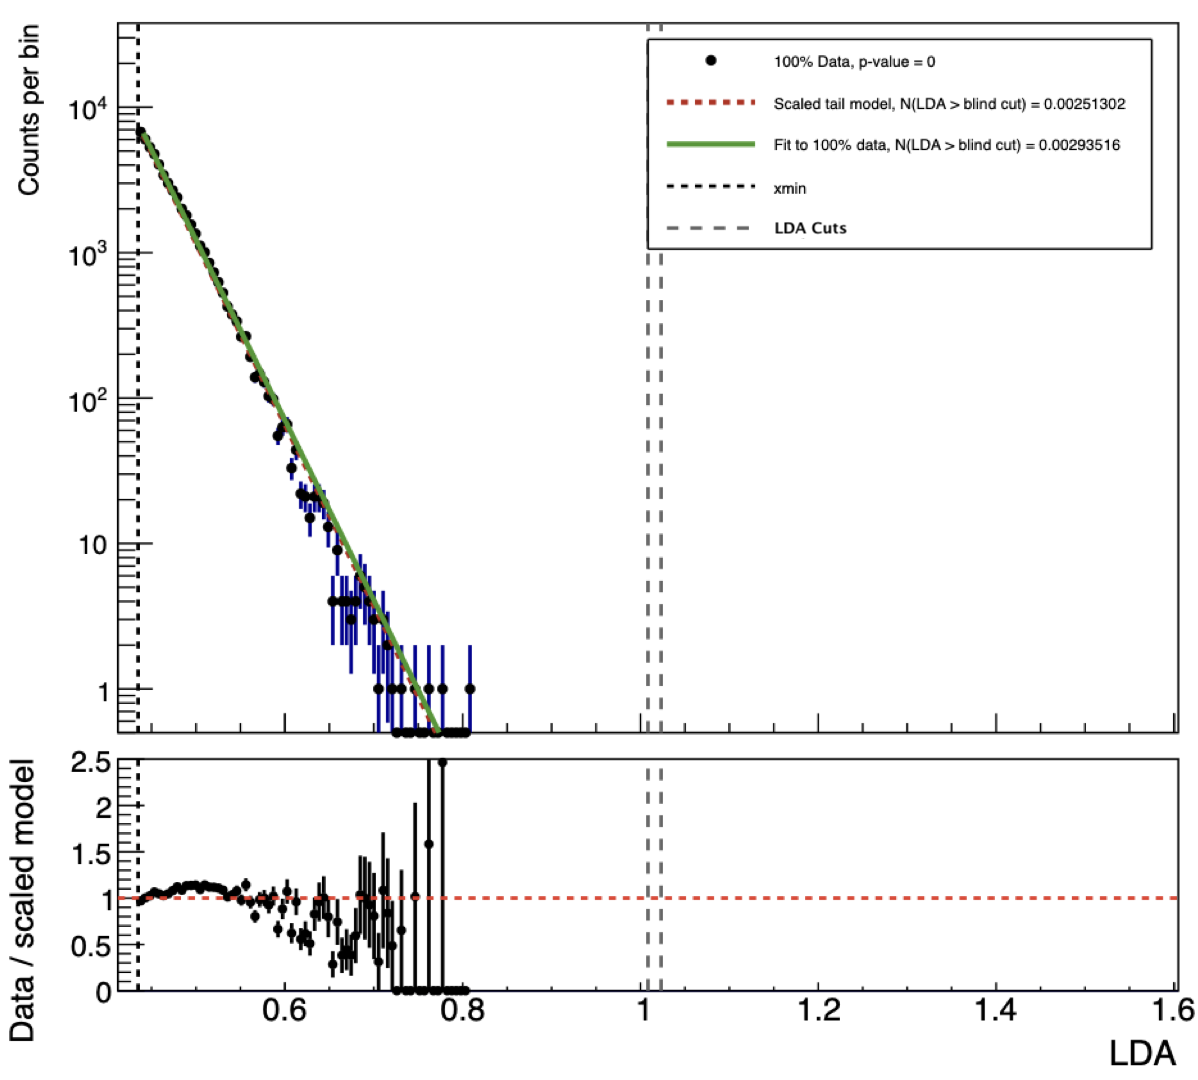
\includegraphics[
          width=0.75\textwidth,
          alt={}
      ]{sections/5sa-analysis/images/a2c4_100pct_lda_backgroundfit.png}
      \caption{
        Top: The distribution of thermal events (events that passed all cuts defined in Chapter~\ref{chap:5sa_cleaning}) from the 100\% sample of A2 configuration 4 (black dots with blue error bars).
        Only events with LDA scores greater than the $x_{\text{min}}$ used to fit the background model in Section~\ref{sec:lda} (black dotted line) and less than the appropriate LDA Cut established in Section~\ref{sec:optimization} are plotted (grey dashed lines).
        These are events are fit to an exponential (green line) plotted along the model built on the 10\% data multiplied by 10 (red dotted line).
        Bottom: Ratio of the 100\% LDA distribution of thermal events (black dots in top panel) divided by the model built on the 10\% data scaled up by a factor of 10 (red dotted line in top panel).
      }
      \label{fig:backgroundcheck_a2c4}
    \end{figure}

    \begin{figure}
      \centering
      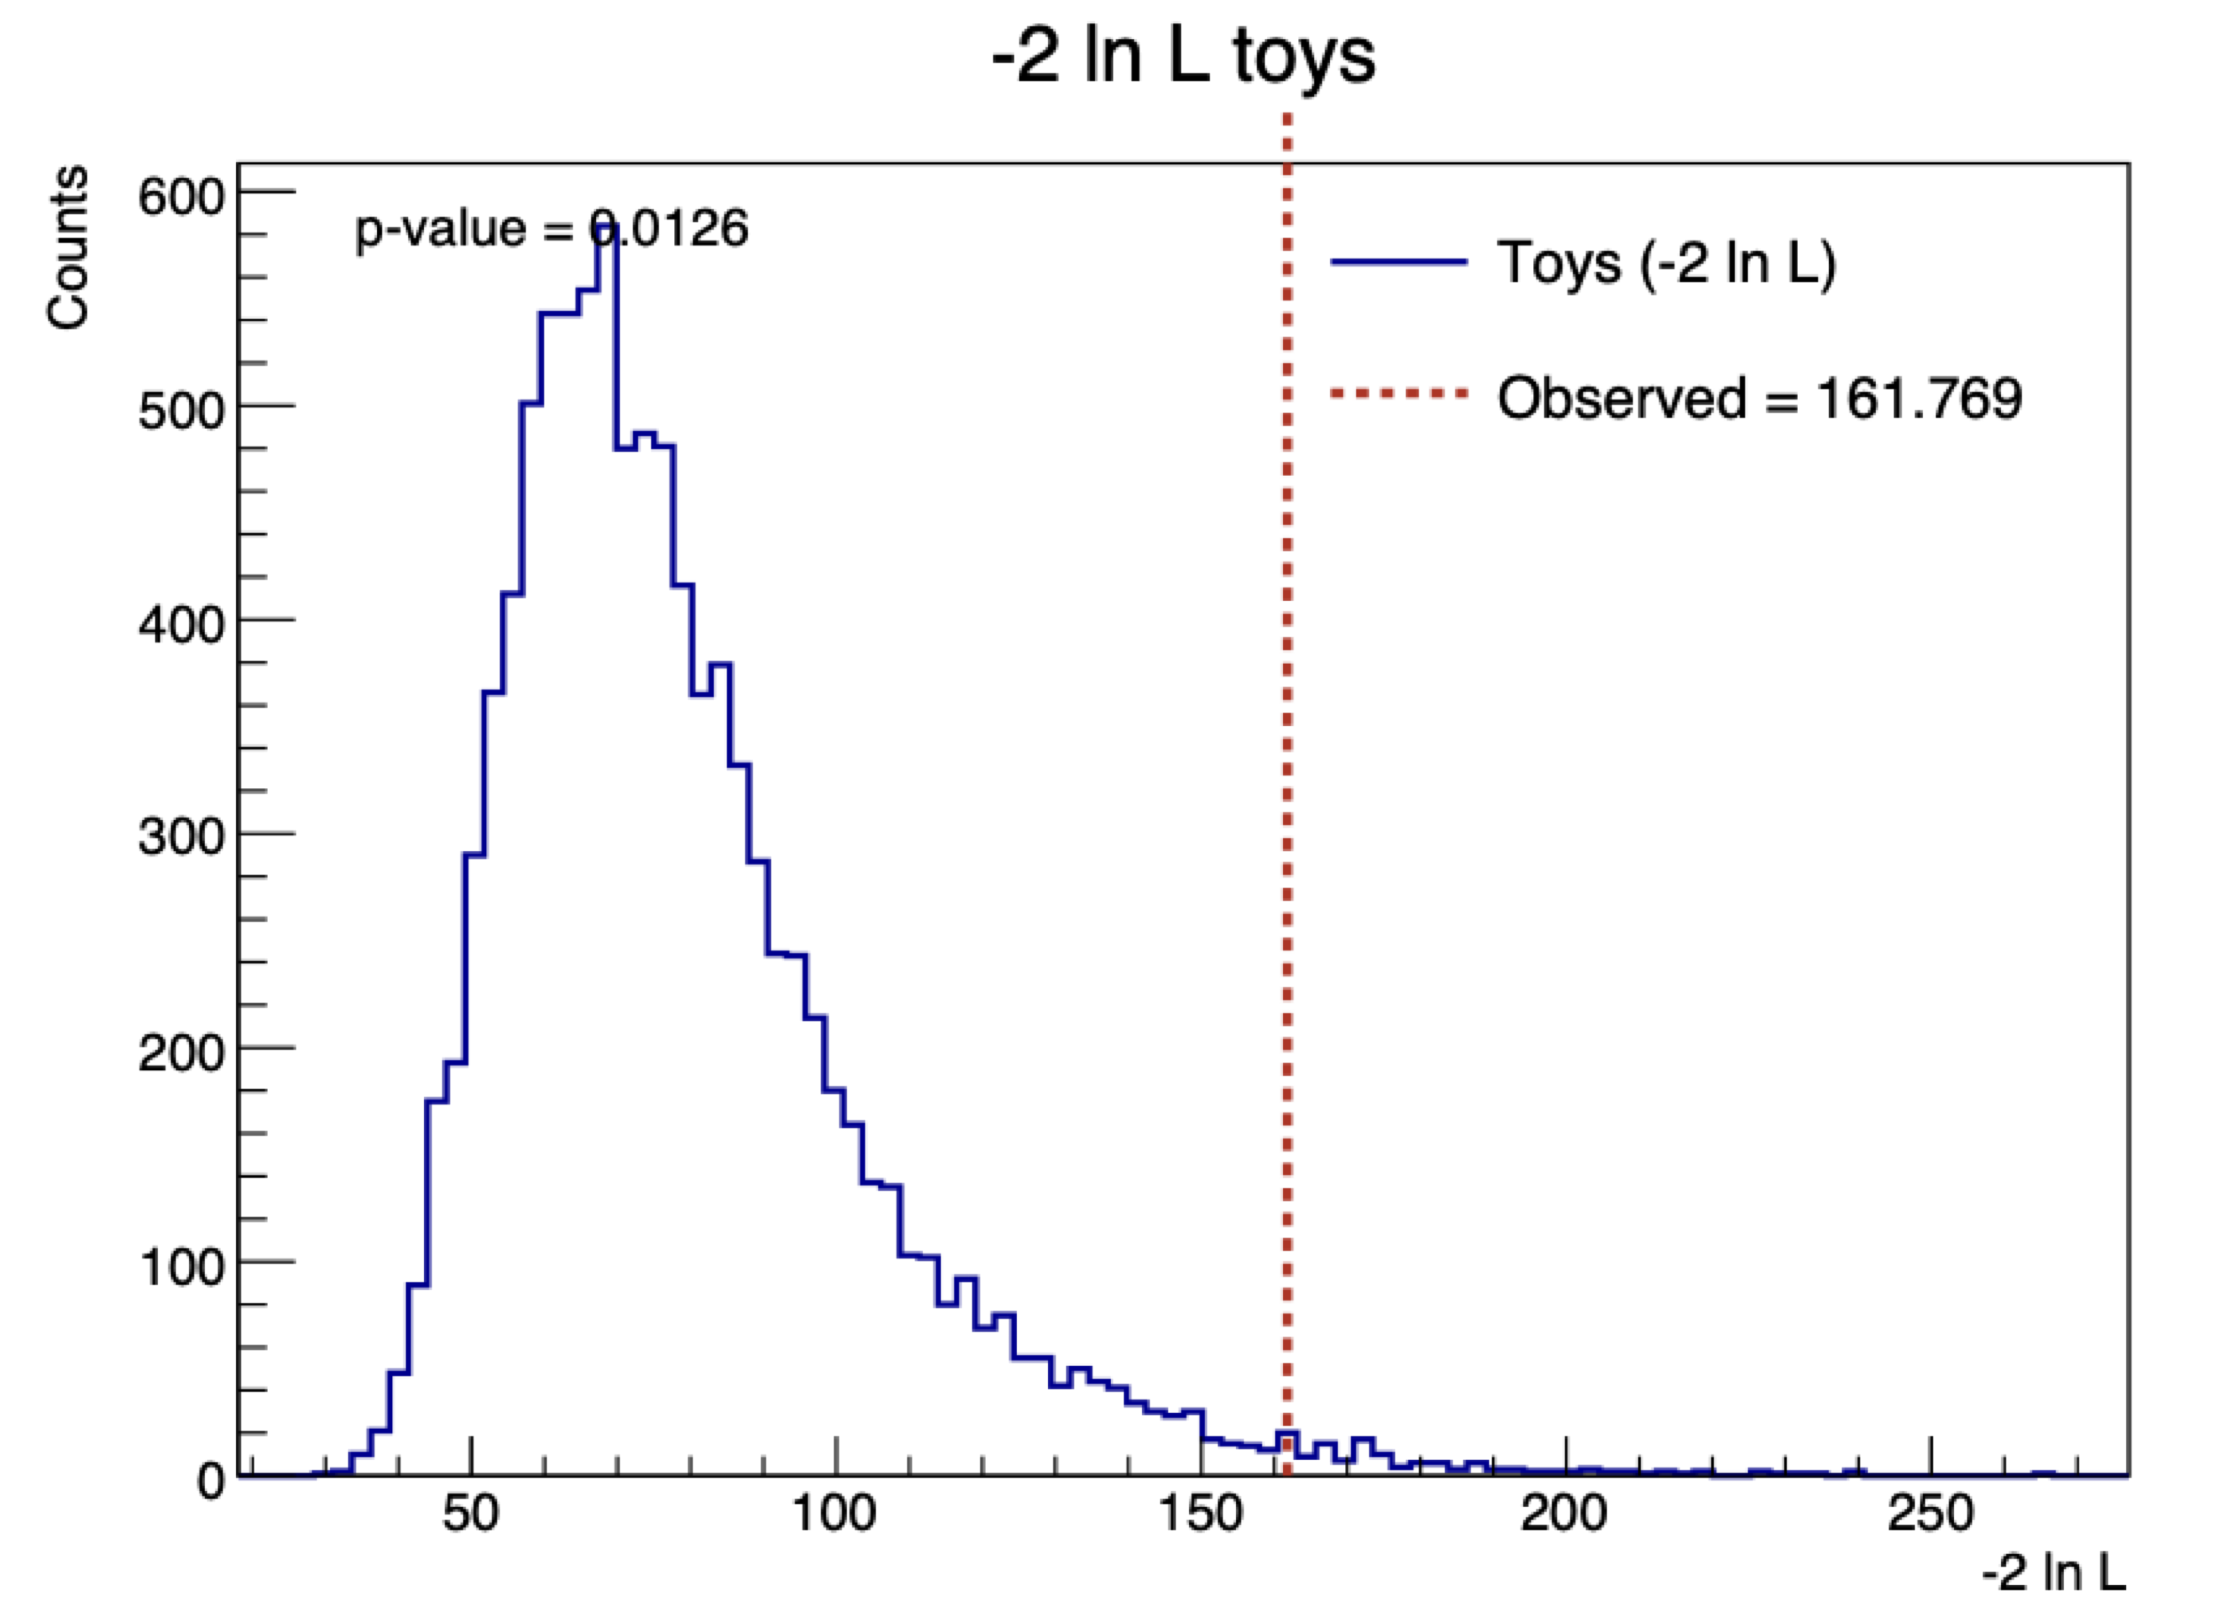
\includegraphics[
          width=0.75\textwidth,
          alt={}
      ]{sections/5sa-analysis/images/a2c3_100pct_lda_backgroundfit_toys.png}
      \caption{
        Distribution of the log-likelihood of pseudoexperiments built on 100\% A2 Configuration 3 data (blue distribution) compared to the log-likelihood of the observed 100\% data (red line) both calculated against the 10\% background model scaled up by a factor of 10.
      }
      \label{fig:backgroundcheck_a2c3_toys}
    \end{figure}

    \begin{figure}
      \centering
      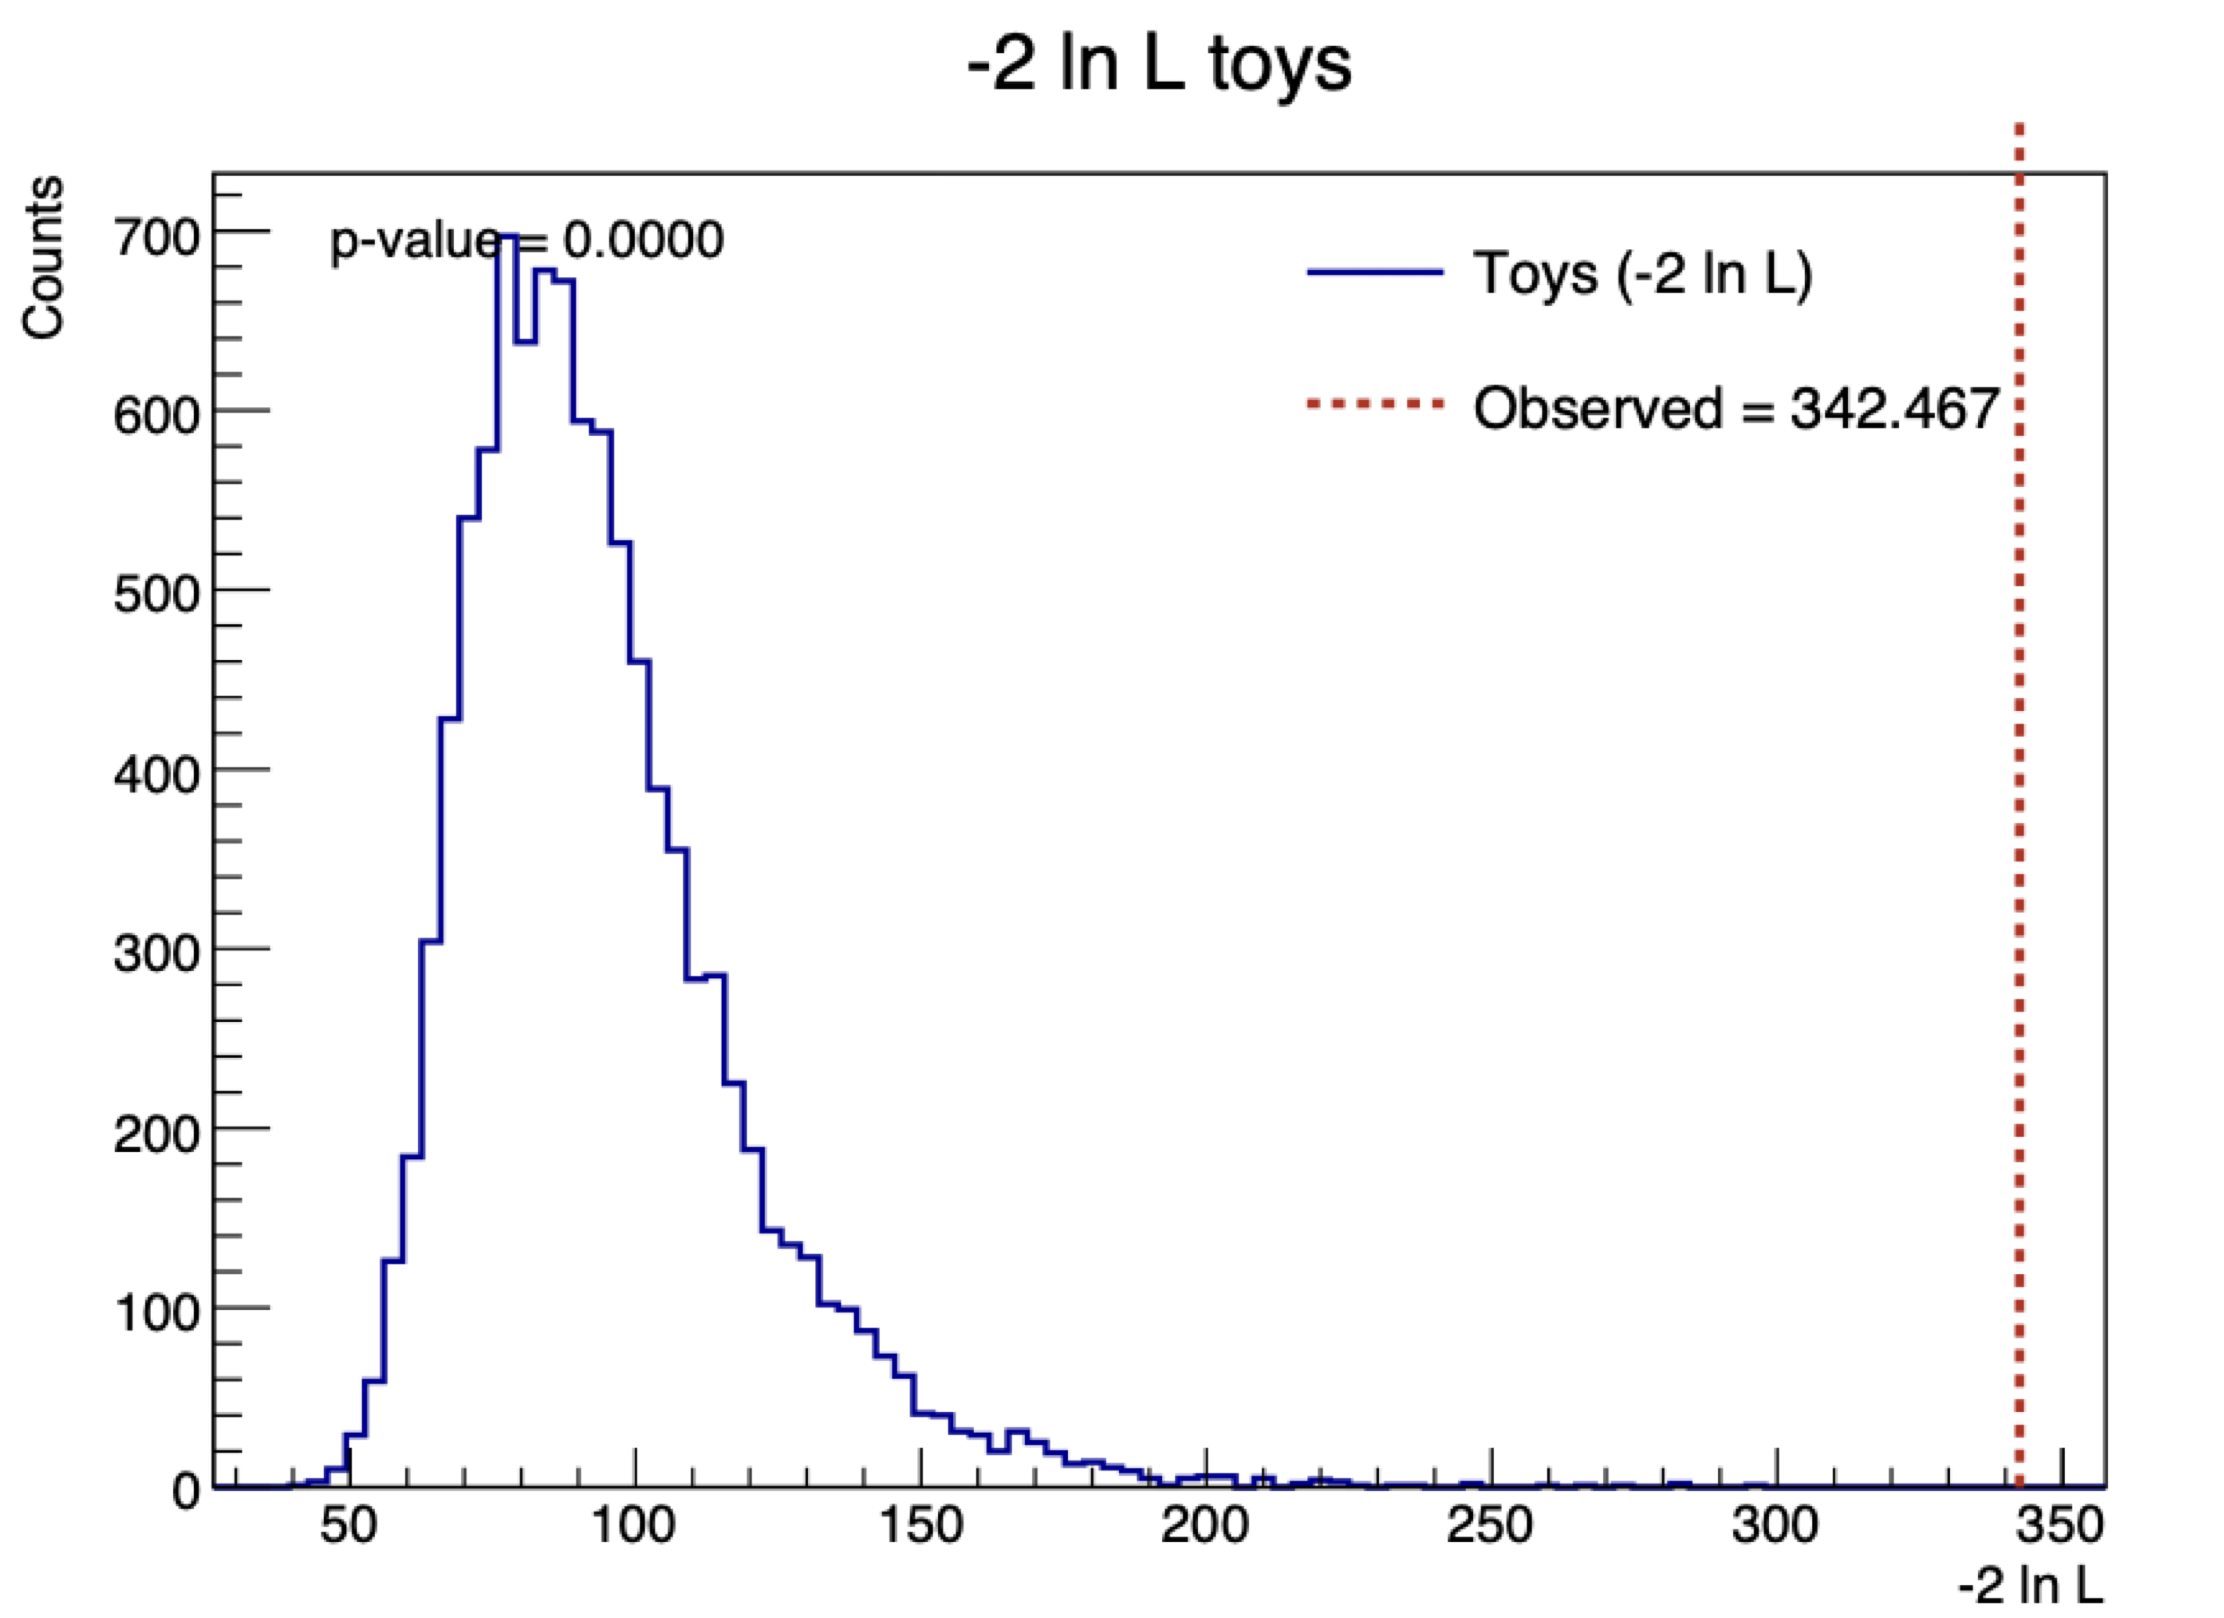
\includegraphics[
          width=0.75\textwidth,
          alt={}
      ]{sections/5sa-analysis/images/a2c4_100pct_lda_backgroundfit_toys.png}
      \caption{
        Distribution of the log-likelihood of pseudoexperiments built on 100\% A2 Configuration 4 data (blue distribution) compared to the log-likelihood of the observed 100\% data (red line) both calculated against the 10\% background model scaled up for a factor of 10.
      }
      \label{fig:backgroundcheck_a2c4_toys}
    \end{figure}

    \begin{figure}
      \centering
      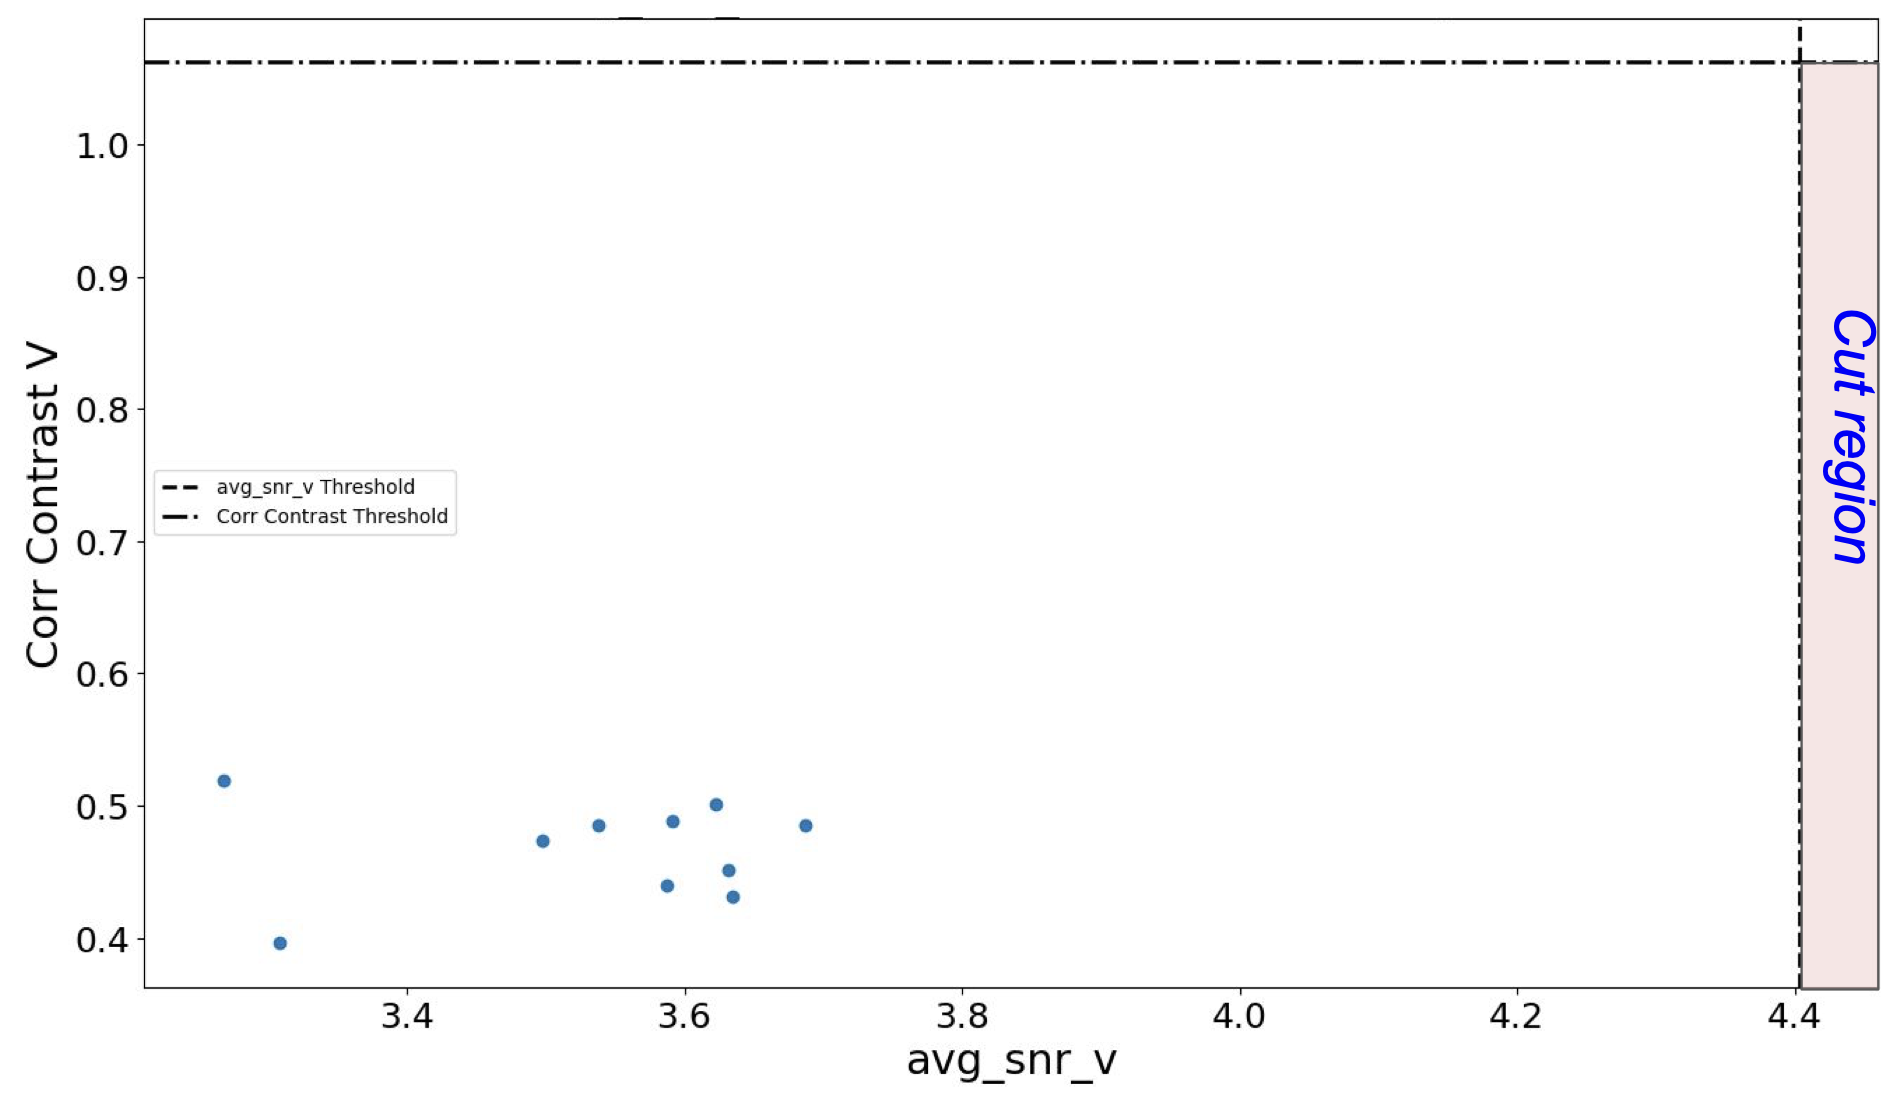
\includegraphics[
          width=0.75\textwidth,
          alt={}
      ]{sections/5sa-analysis/images/a2c3_100pct_lda_backgroundfit_outliers.png}
      \caption{
        Events from the A2 Configuration 3 distribution plotted in Fig.~\ref{fig:backgroundcheck_a2c3} with the highest LDA scores plotted by \texttt{corr\_contrast\_v} (relating the maximum reconstruction correlation score to the average) against \texttt{avg\_snr\_v} (signal strength).
        These are the variables used in the Low Reconstruction Confidence Cut defined in Section~\ref{sec:lrcc}. 
        The events plotted have \texttt{corr\_contrast\_v} well within the range the Low Reconstruction Confidence Cut isolates events for, but the \texttt{avg\_snr\_v} scores were too low for the events to be cut. 
        These events are therefore just thermal outliers with no indication that they are signal-like and would corrupt our background model.
      }
      \label{fig:backgroundcheck_a2c3_outliers}
    \end{figure}

    \begin{figure}
      \centering
      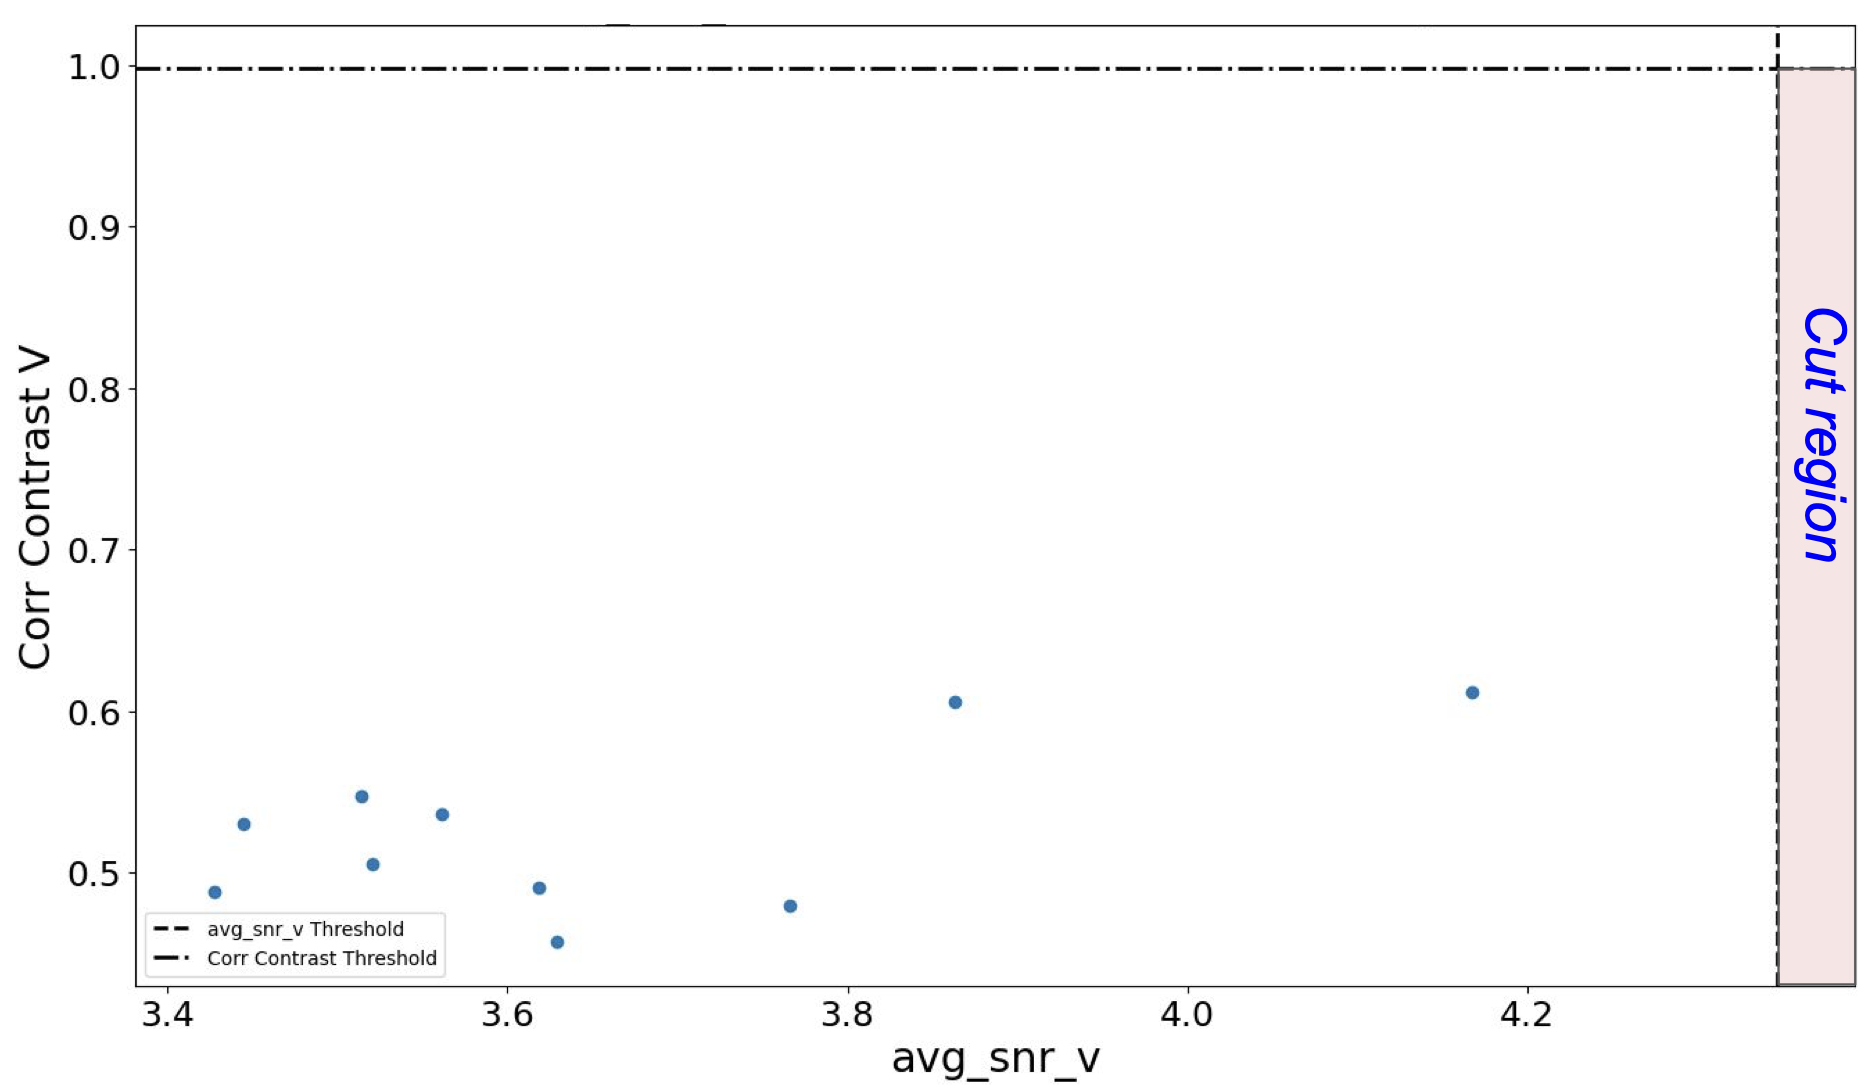
\includegraphics[
          width=0.75\textwidth,
          alt={}
      ]{sections/5sa-analysis/images/a2c4_100pct_lda_backgroundfit_outliers.png}
      \caption{
        Events from the A2 Configuration 4 distribution plotted in Fig.~\ref{fig:backgroundcheck_a2c3} with the highest LDA scores plotted by \texttt{corr\_contrast\_v} (relating the maximum reconstruction correlation score to the average) against \texttt{avg\_snr\_v} (signal strength).
        These are the variables used in the Low Reconstruction Confidence Cut defined in Section~\ref{sec:lrcc}. 
        The events plotted have \texttt{corr\_contrast\_v} well within the range the Low Reconstruction Confidence Cut isolates events for, but the \texttt{avg\_snr\_v} scores were too low for the events to be cut. 
        These events are therefore just thermal outliers with no indication that they are signal-like and would corrupt our background model.
      }
      \label{fig:backgroundcheck_a2c4_outliers}
    \end{figure}

    To investigate the low p-value on A2 configuration 3 and configuration 4, we first looked for run-level anomalies then looked at each event driving the disagreement between the 10\% model and the 100\% model.
    For configuration 3, we identified runs that had unstable firmware (6558-6569) and poor restabilization after a reported power fail (7100), all of which should have been in the Bad Run Log.
    We then established that all remaining events would have been cut by the Low Reconstruction Confidence Cut described in Section~\ref{sec:lrcc} if these events had been more signal-like, meaning these events were determined to be thermal-like but were upward fluctuations of the backgrounds enough to invalidate the background model, as shown in Fig.~\ref{fig:backgroundcheck_a2c3_outliers}.
    All outliers in the configuration 4 background LDA model were similar, they would have been removed by the Low Reconstruction Confidence Cut if they had been more signal-like, as shown in Fig.~\ref{fig:backgroundcheck_a2c4_outliers}. 
    These outliers were therefore deemed inconsequential and, after adding those runs to the Bad Run Log and therefore excluding these events from analysis, the 100\% background fit to configurations 3 and 4 were deemed to be compatible with the 10\% fits. 

  \subsection{Time Isolation Cut}

    As neutrinos are expected to be rare, it is even rarer that multiple diffuse neutrino observations would occur within a short time window. 
    To avoid collections of temporally clustered, unanticipated, neutrino-like background events from passing this analysis, we enforce a Time Isolation Cut to remove events that pass all cuts but occur within a short time window. 
    This time window was determined via a toy Monte Carlo simulation which sampled a number of neutrino events from a Poisson distribution with a mean of 15 and randomly distributed these events over the 10.6 year livetime covered by this analysis. 
    The time between consecutive events was calculated for all trials and plotted in Figure~\ref{fig:isolation_condition}.
    The time window with less than a 0.001\% probability of removing neutrinos was 5.8 hours and is used to defined the Time Isolation Cut window.

    \begin{figure}
        \centering
        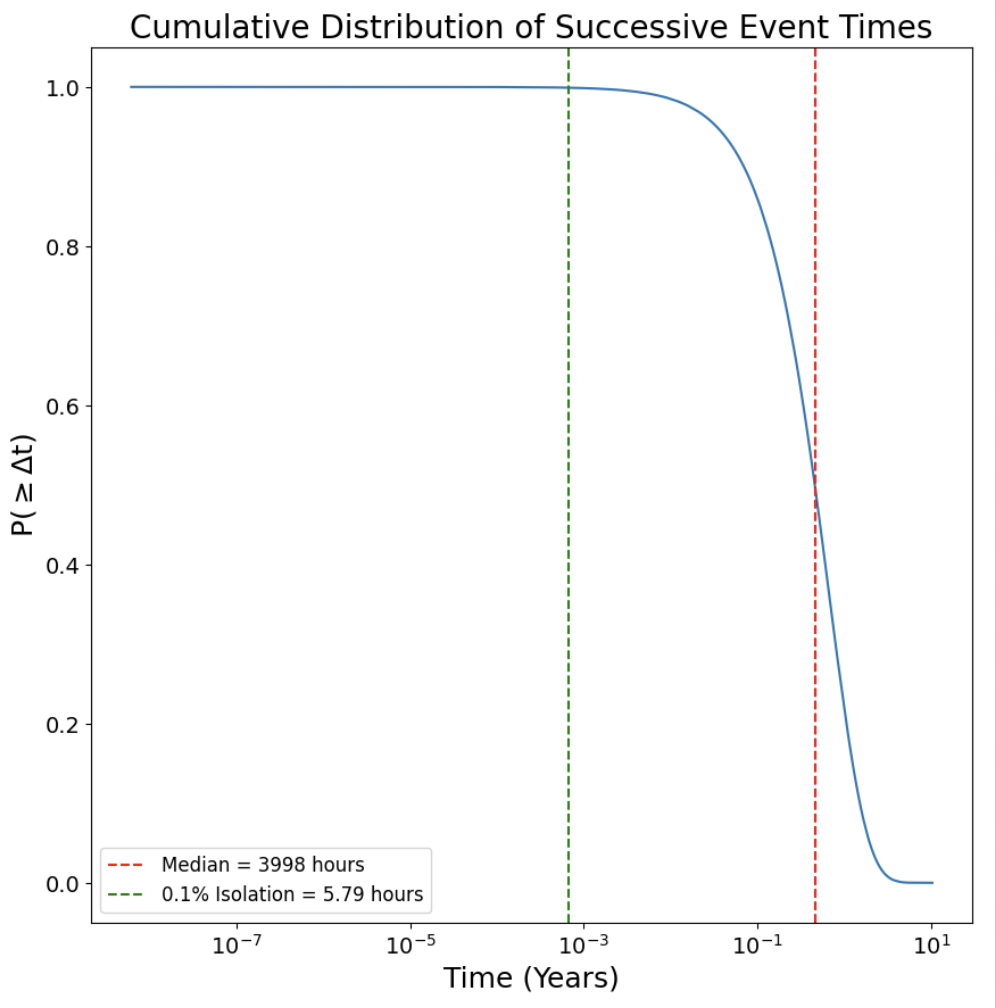
\includegraphics[
            width=0.75\textwidth,
            alt={}
        ]{sections/5sa-analysis/images/isolation.png}
        \caption{
          Cumulative distribution of the time difference between successive events in the toy Monte Carlo simulation of neutrino event detection times (blue).
          The average time separation between successive neutrino events is 3998 hours (red, 5.48 months).
          99.9\% of events occur at least 5.79 hours apart (green).
        }
        \label{fig:isolation_condition}
    \end{figure}

    However, this analysis considers neutrino events that may involve multiple cascades resulting from muon stochastic losses, tau stochastic losses, and tau decays. 
    We expect that these types of events will not trigger the same detector twice very often, given the lengthy, $\mathcal{O}(\text{1 ms})$ deadtime of ARA stations and geometric constraints of Askaryan radiation, but in Figure~\ref{fig:multistation} we showed that we expect multiple stations to observe one or more cascades resulting from $10^{19}$~eV neutrinos 10\% of the time, increasing to 35\% for neutrinos with $10^{21}$~eV of energy.
    We therefore retain passing event multiplets within a time window of 5~s. 

\pagebreak
\section{Inspection of Passing Events \label{sec:passing_events}}

    As this type of experiment and analysis expects to observe 0 or 1 event on a background of $\sim\!0$ events, any events that pass all analysis cuts will need to be assessed to determine if they are consistent with simulated neutrino events or some unanticipated technical background. 
    The analysis will not be substantially changed, however a posteriori inspection of any new backgrounds may warrant an update to the analysis cuts. 
    This should be performed in a regimented way and cuts should only be made more conservative.

    \subsection{Approach to Analyzing Unblinded Data}

      For any events that pass all analysis cuts, our goal is to analyze all analysis variables for the events before consulting the waveform and reconstruction skymap - preserving analysis ``blindness'' as long as possible. 
      Some examples of first stage analyzes include analyzing the time each event occurred, the reconstructed azimuth and elevation of events, conducting a KS test for azimuthal randomness, and consulting analysis variables associated with the Spark Event Cut and Anomalous Channel Cut which identify glitches. 
      If more information is needed, we will then consult the event waveforms, spectra, and reconstruction skymaps. 
      We expect that the only events that pass the analysis will be neutrino candidates.
      If a population of events passes the analysis and is subsequently determined to be inconsistent with our expectation of neutrino observations, appears to be a new class of unanticipated glitches or unexpected technical background, and can be removed in a principled fashion, then we will employ a new cut and the events will not be included in the upcoming Feldman Cousins factor calculation that determines the upper limit set by the analysis. 
      Any remaining events will be assessed for compatibility with our expectation of neutrino observations. % How is this different from an LDA? why didn't we use this instead of the LDA?
      If any events are more consistent with background than expected neutrino events, we will update our background estimate if the Poisson p-value to observe such an upward fluctuation is greater than $3\sigma$.

      Ultimately, the number of events that pass this analysis and that cannot be explained as an unanticipated background will contribute to the number of observed neutrino candidates by this analysis.
      This will be used to calculate the neutrino flux or upper limit on the neutrino flux in Section~\ref{sec:5sa_results}.

    \subsection{A Posterior Investigation of the Passing Event}

      The results of the analysis on the 100\% revealed a single passing event taken by the Phased Array (PA). 
      As only one event was found, no events were cut by the Time Isolation Cut. 
      After analyzing the event, we determined that it was a glitch.
      Furthermore, we identified that this class of events is a type of technical background that has been observed on stations A1-A5.
      Two dedicated cuts were already developed and used to address this class of events, the Spark Event Cut and the Anomalous Channel Cut.
      Earlier investigations assumed the malfunction was on the data acquisition (DAQ) board of A1-A5 which would not affect the PA which has a different DAQ board.
      However, closer inspection of this event indicated downhole electronics emitted radiation.
      This causes the waveforms of some channels to saturate while simultaneously generating radio-wavelength emission that is observed by nearby antennas.
      This means that glitches on A5 strings can be observed by the PA.
      We have not seen this glitch occur on the PA string.
      Given this new understanding, we expanded the cuts to remove PA events within 0.1~s of A5 events removed by the Spark Event Cut and the Anomalous Event Cut. 
      This removes the passing event so it will not be included in the Feldman Cousins upper limit calculation.
      The rest of this section details the study of this event following the prescription outlined in the previous section and how we determined this event was caused by a glitch. 

      \begin{figure}
        \centering
        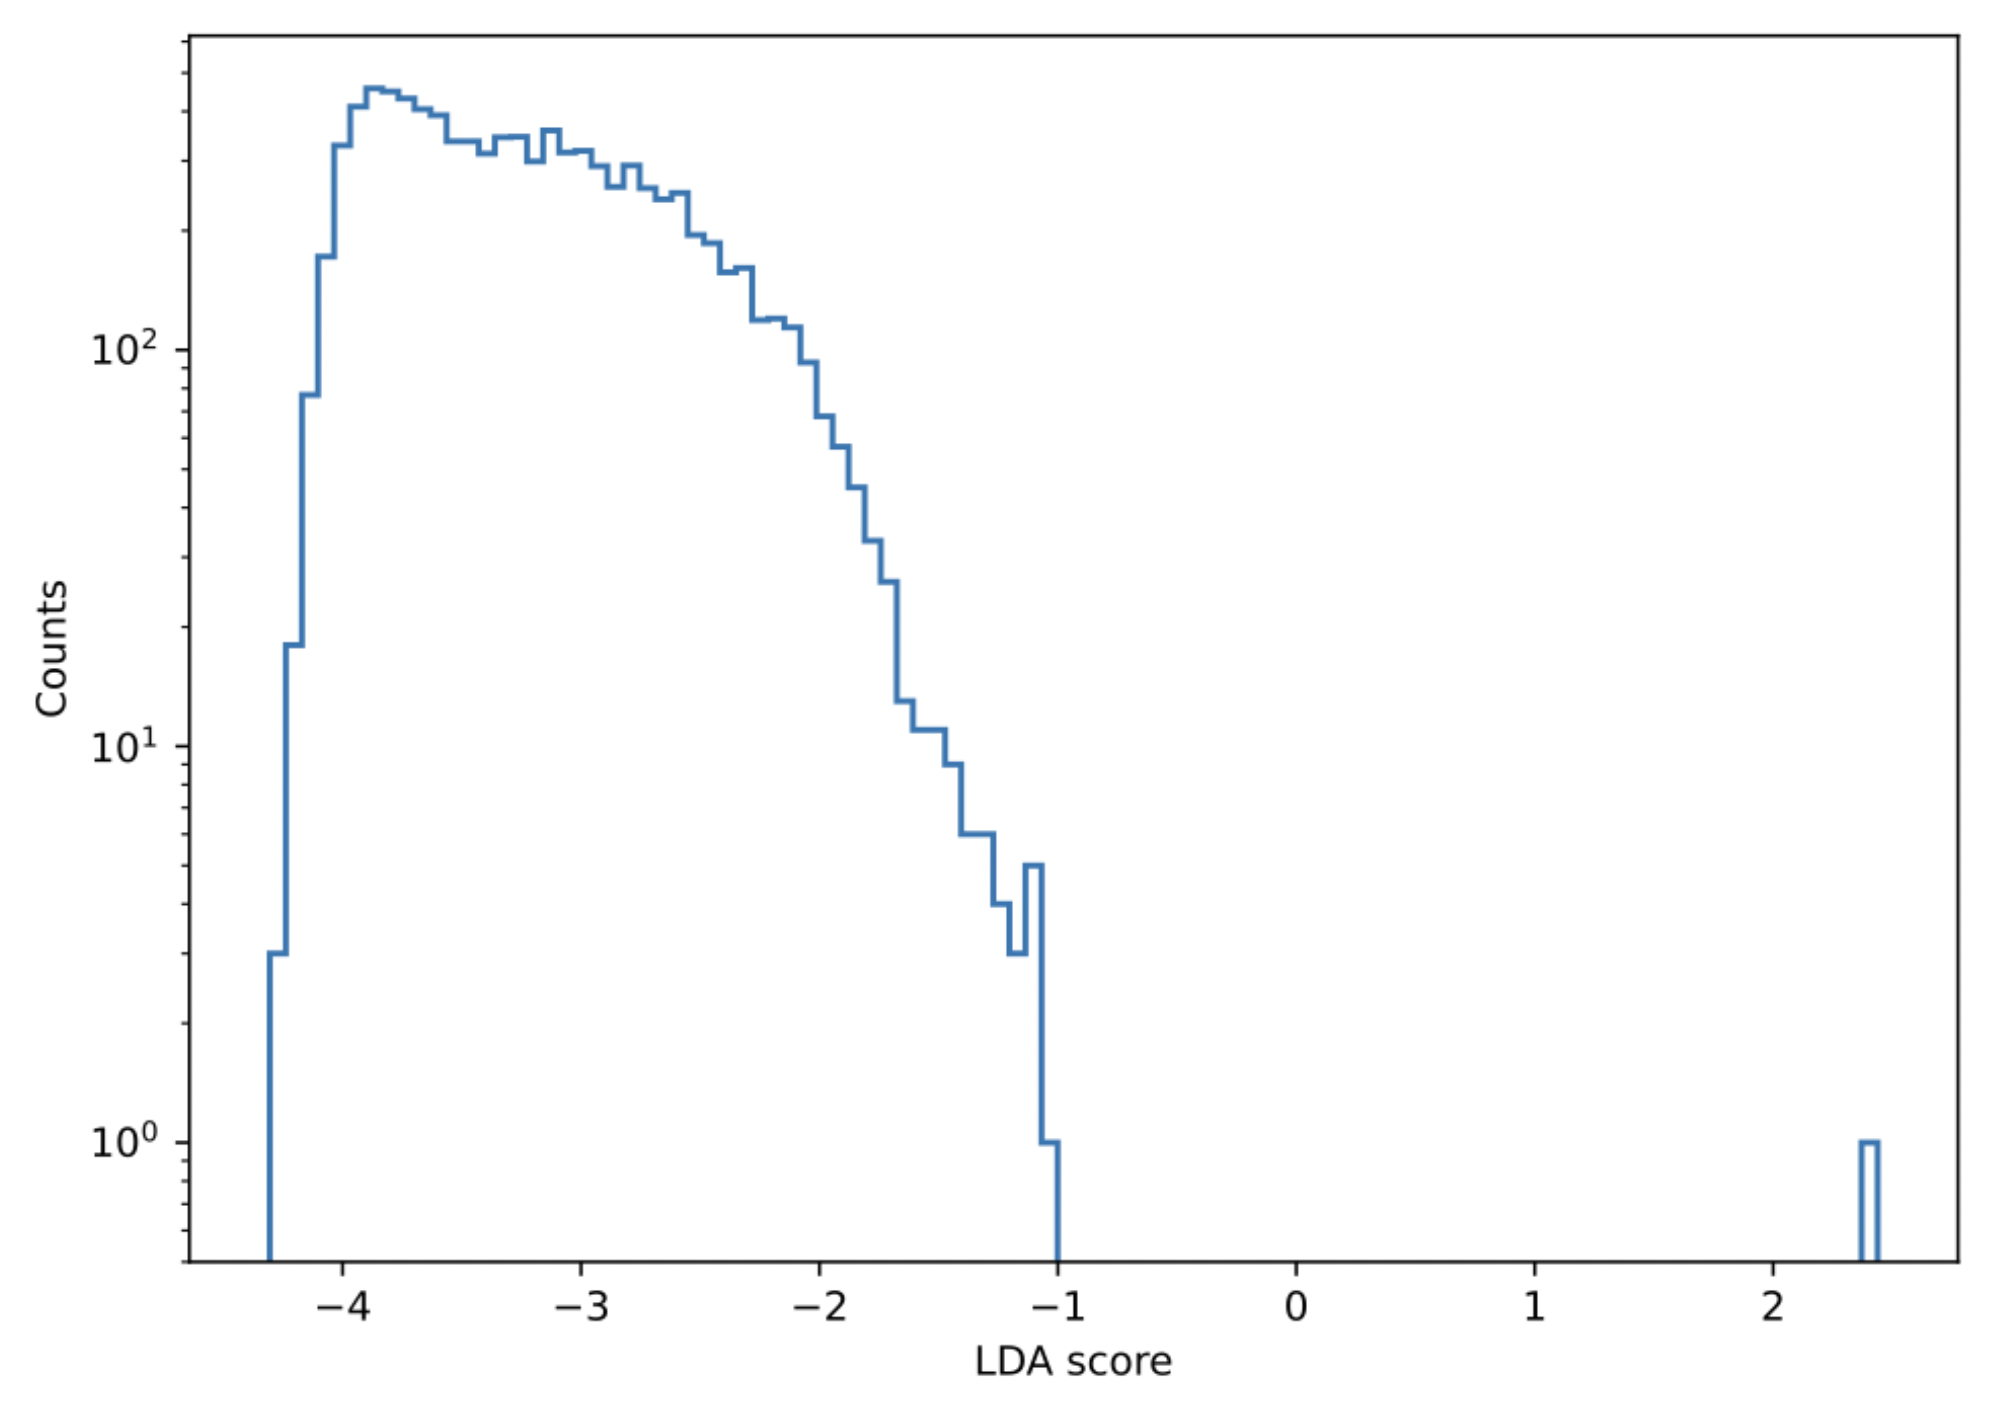
\includegraphics[
          width=0.7\linewidth,
          alt={}
        ]{sections/5sa-analysis/images/passing_lda_parun767.png}
        \caption{
          LDA distribution of events in PA run 767. The event that passed the analysis is the outlier with an LDA score of 2.43 and the LDA cut for this configuration was 1.17.
        }
        \label{fig:passing_LDA}
      \end{figure}

      The passing event's LDA score was 2.43 and was a significant outlier to the rest of the events in the run, as shown in Figure~\ref{fig:passing_LDA}.
      Some analysis variables of the PA event are presented in Table~\ref{tab:paevent} but the full suite is provided in Appendix~\ref{app:pa_passingevent}. 
      In short, this event
      \begin{itemize}
        \item was taken on April 4, 2018 at 06:01:17 UTC,
        \item saturated the PA DAQ when it was recorded,
        \item observed an SNR of 12.5 in the VPols, and
        \item observed an SNR of 11.8 in the HPols.
      \end{itemize}
      The event reconstructs to an elevation of $-35^{\circ}$ and, from the \texttt{mindepth\_v}, indicates that the highest elevation with a reconstruction correlation score that is 60\% of the maximum lies at an elevation angle of $-27.6^{\circ}$.
      This reconstruction is of good quality and suggests an in-ice origin for this signal.

      \begin{table}
        \centering
        \begin{tabular}{
          | >{\centering\arraybackslash}m{3.5cm}  
          | >{\centering\arraybackslash}m{3.5cm}  
          | >{\centering\arraybackslash}m{2.5cm}  
          >{\centering\arraybackslash}m{3.5cm}  |
        }
          \hline
          PA Analysis Variable & Corresponding AraProc Analysis Variable & Value & Note \\
          \hline
          \texttt{avgHpolSnr} & \texttt{avg\_snr\_h} & 11.78 &  \\
          \texttt{avgPaSnr} & \texttt{avg\_snr\_v} & 12.46 &  \\
          \texttt{avgRms} & \texttt{avg\_rms\_v} & 57.71 V &  \\
          \texttt{bestCorr} & \texttt{global\_max\_corr} & 0.18 &  \\
          \texttt{bestPhi} & \texttt{global\_max\_phi} & 5.67 rad &  \\
          \texttt{bestTheta} & \texttt{global\_max\_theta} & 2.18 rad & Elevation angle \\
          \texttt{corrContrast} & \texttt{corr\_contrast\_v} & 7.01 &  \\
          \texttt{cswPaSnr} & \texttt{csw\_snr\_v} & 12.89 &  \\
          \texttt{eventNo} & \texttt{event\_number} & 89985 &  \\
          \texttt{imp} & \texttt{impulsivity\_v} & 0.81 &  \\
          \texttt{ldaScore} & \texttt{} & 2.44 &  \\
          \texttt{runNo} & \texttt{run\_number} & 767 &  \\
          \texttt{s2} & \texttt{avg\_s2\_v} & 11.25 &  \\
          \texttt{unixTime} & \texttt{unixtime} & 1522821677 &  \\
          \hline
        \end{tabular}
        \caption{
          Analysis variables for the passing event calculated using the PA analysis framework, the corresponding analysis variable calculated by AraProc, the value of the PA analysis variable, and any notes regarding the variable.
        }
        \label{tab:paevent}
      \end{table}

      \begin{figure}
        \centering
        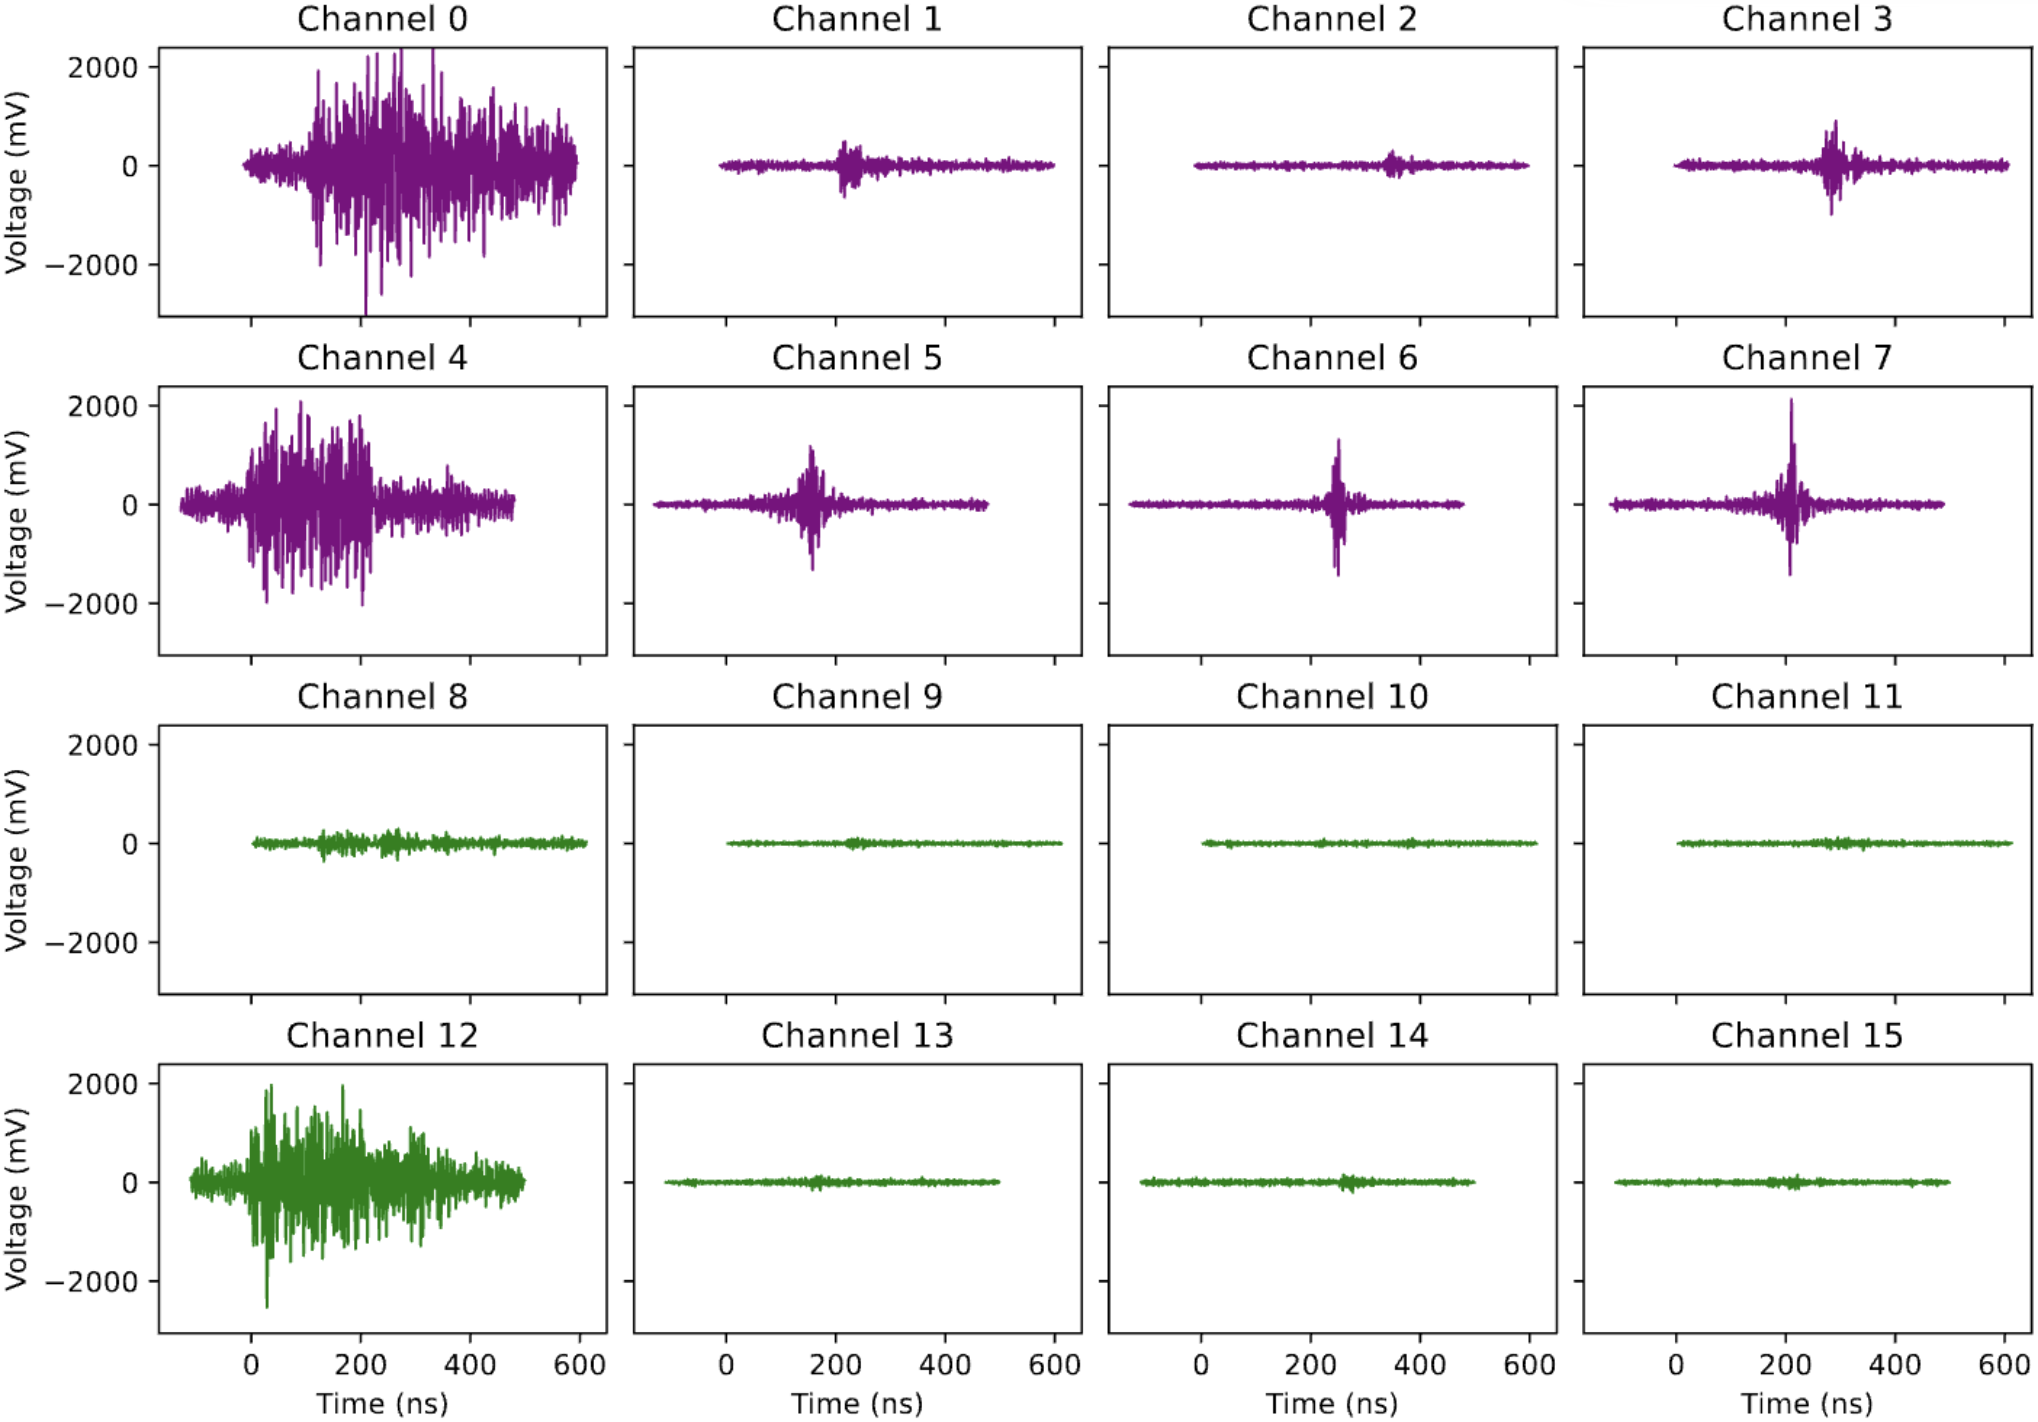
\includegraphics[
          width=\linewidth,
          alt={}
        ]{sections/5sa-analysis/images/passingevent_a5waveform.png}
        \caption{
          The voltage versus time waveforms in each A5 antenna for event 64066 of Run 2899, the A5 event corresponding to the PA event that passed the analysis.
          The high root-mean-square voltage observed in Channel 0, 4, and 12 (which are all located on the same string) is a typical feature of the events removed by the Anomalous Channel Cut defined in Section~\ref{sec:acc}.
          Impulsive signals are also visible on the three other A5 strings.
        }
        \label{fig:passing_a5waveform}
      \end{figure}

      The PA is colocated with A5 and an A5 event was recorded at the same time as this passing PA event.
      % As discussed in Section~\ref{sec:triggering}, signals that trigger both A5 and the PA trigger A5 first
      The A5 event was removed from the analysis by the Anomalous Channel Cut and indicate anomalous waveforms incompatible with expectations of a neutrino observation.
      Figure~\ref{fig:passing_a5waveform} shows high root-mean-square voltage in channels 0, 4, and 12 and impulsive signatures on strings 2, 3 and 4 of the A5 event. 
      The characteristics of these waveforms are consistent with the A4 event that inspired the Anomalous Channel Cut\index{Cut, Anomalous Channel} as described in Section~\ref{sec:acc}.

      We also looked for events in stations A1-A4 that occurred within 24 hours of the passing PA event. 
      We found no events in A1-A3 and one event in A4 that occurred within 0.5~seconds of the PA and A5 events. 
      This A4 event was also the same event from the 10\% sample that motivated the creation of the Anomalous Channel cut. 
      The A4 event is shown in Figure~\ref{fig:a4outlier} demonstrating the same waveform characteristics as the A5 event shown in Figure~\ref{fig:passing_a5waveform}- one string has multiple antenna waveforms demonstrating power surges and impulsive signatures on the remaining strings.
      There were no activities or occurrences that could explain the A4, A5, and PA events with our current understanding, including ARA monitoring activities, IceCube activities, activation of the radio pulsers at the top of the IceCube volume, South Pole Station activities, and natural phenomena (e.g. earthquakes, solar activity, etc)

      % Our list was as follows: 
      % \begin{itemize}
      %   \item Do all waveforms have a pulse?
      %   \item Do the spectra resemble Askaryan radiation?
      %   \item Are all waveforms similar?
      %   \item Do any channels have waveforms similar to channels 0, 4, 12 in the coincident A5 event shown in Fig.~\ref{fig:passing_a5waveform}?
      % \end{itemize}
      The waveform for the PA passing event is shown in Fig.~\ref{fig:passing_pawaveform}. 
      Immediately, we see that each waveform has a clear pulse, they all look similar, and none resemble channels 0, 4, and 12 in the A5 passing event.
      The PA waveforms all look similar to the waveforms observed by A5 strings 2, 3, and 4 - resembling calibration pulsers, like the one shown in Figure~\ref{fig:noiseevent}. 
      However, the A5 event does not reconstruct into the region where calibration pulsers lie.

      \begin{figure}
        \centering
        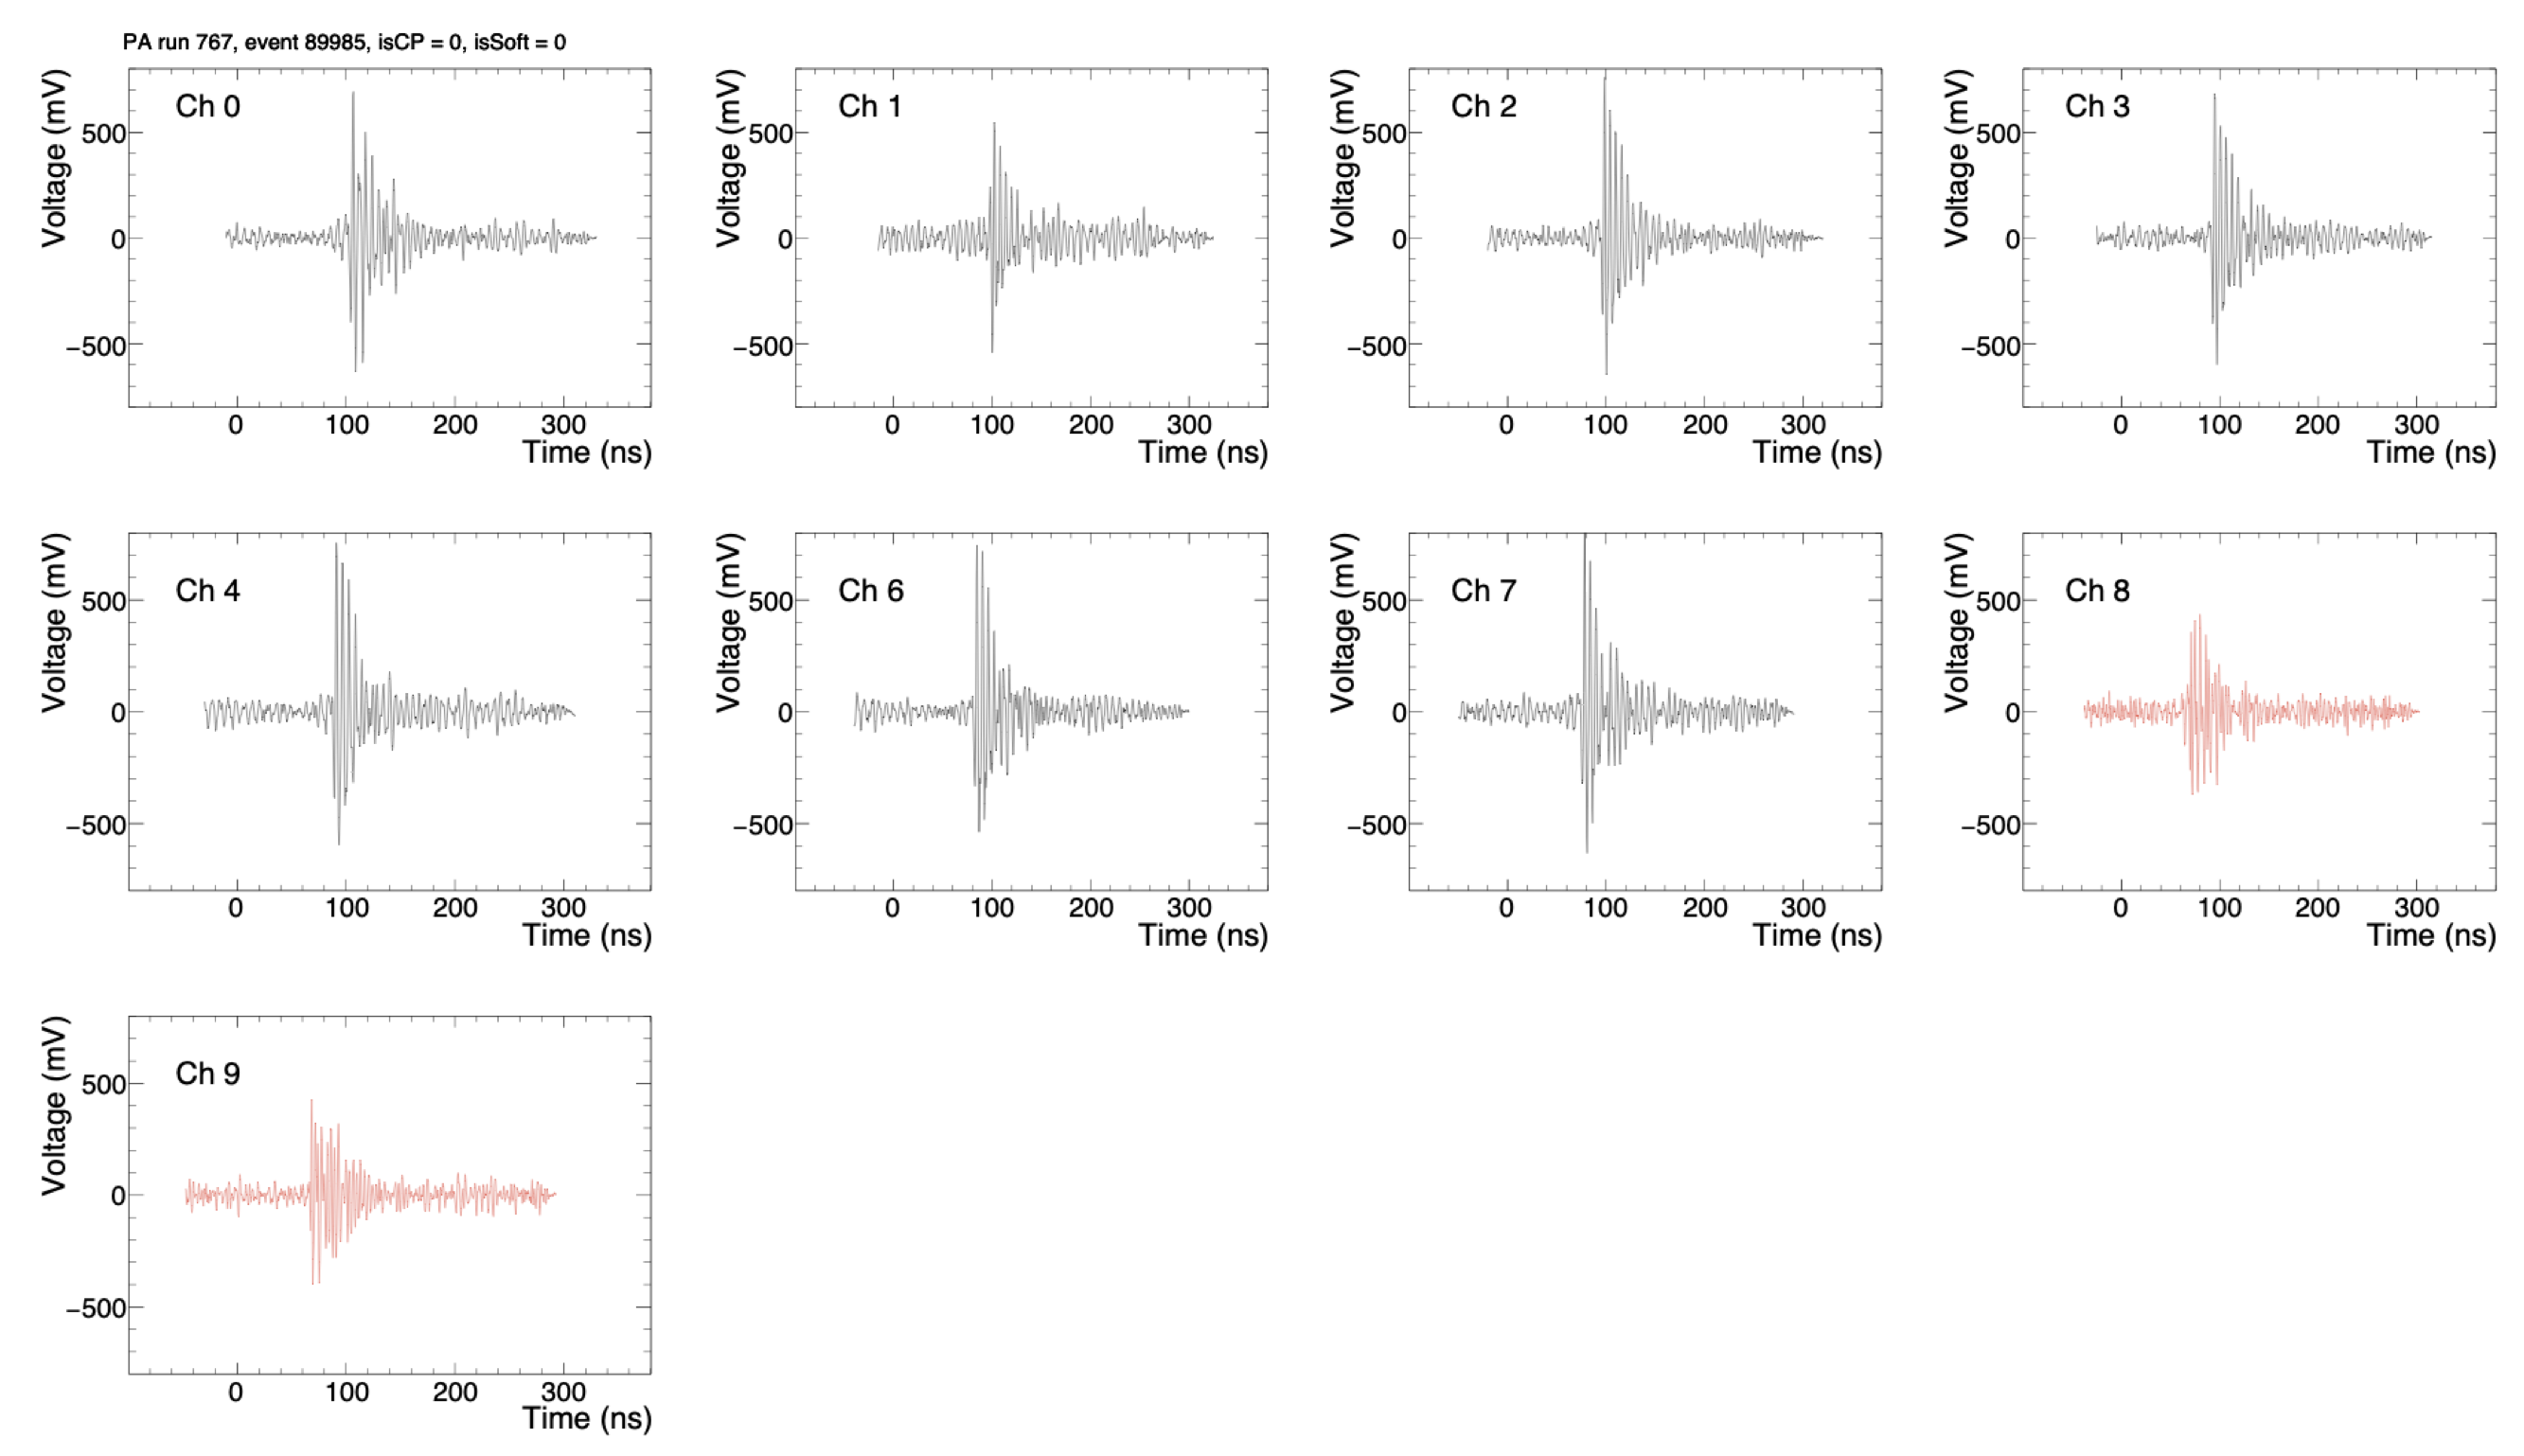
\includegraphics[
          width=\linewidth,
          alt={}
        ]{sections/5sa-analysis/images/passing_pawaveform.png}
        \caption{
          The voltage versus time waveforms in each PA antenna for event 89985 of Run 767, the event that passed the analysis.
          Channel 0 is the top antenna of the PA string and channel 9 is the bottom antenna.
          Channels 0-7 (black) are the vertically polarized antennas from which we construct the PA trigger. 
          Channel 8 and channel 9 (red) are the horizontally polarized antennas at the bottom of the PA string used to enhance angular event reconstruction.
          % This is bandpassed
        }
        \label{fig:passing_pawaveform}
      \end{figure}

      % \comment{I could show the PA event's spectrum and compare it to a calibration pulser but I'd need to ask Marco to generate it for me.}

      \begin{figure}
        \centering
        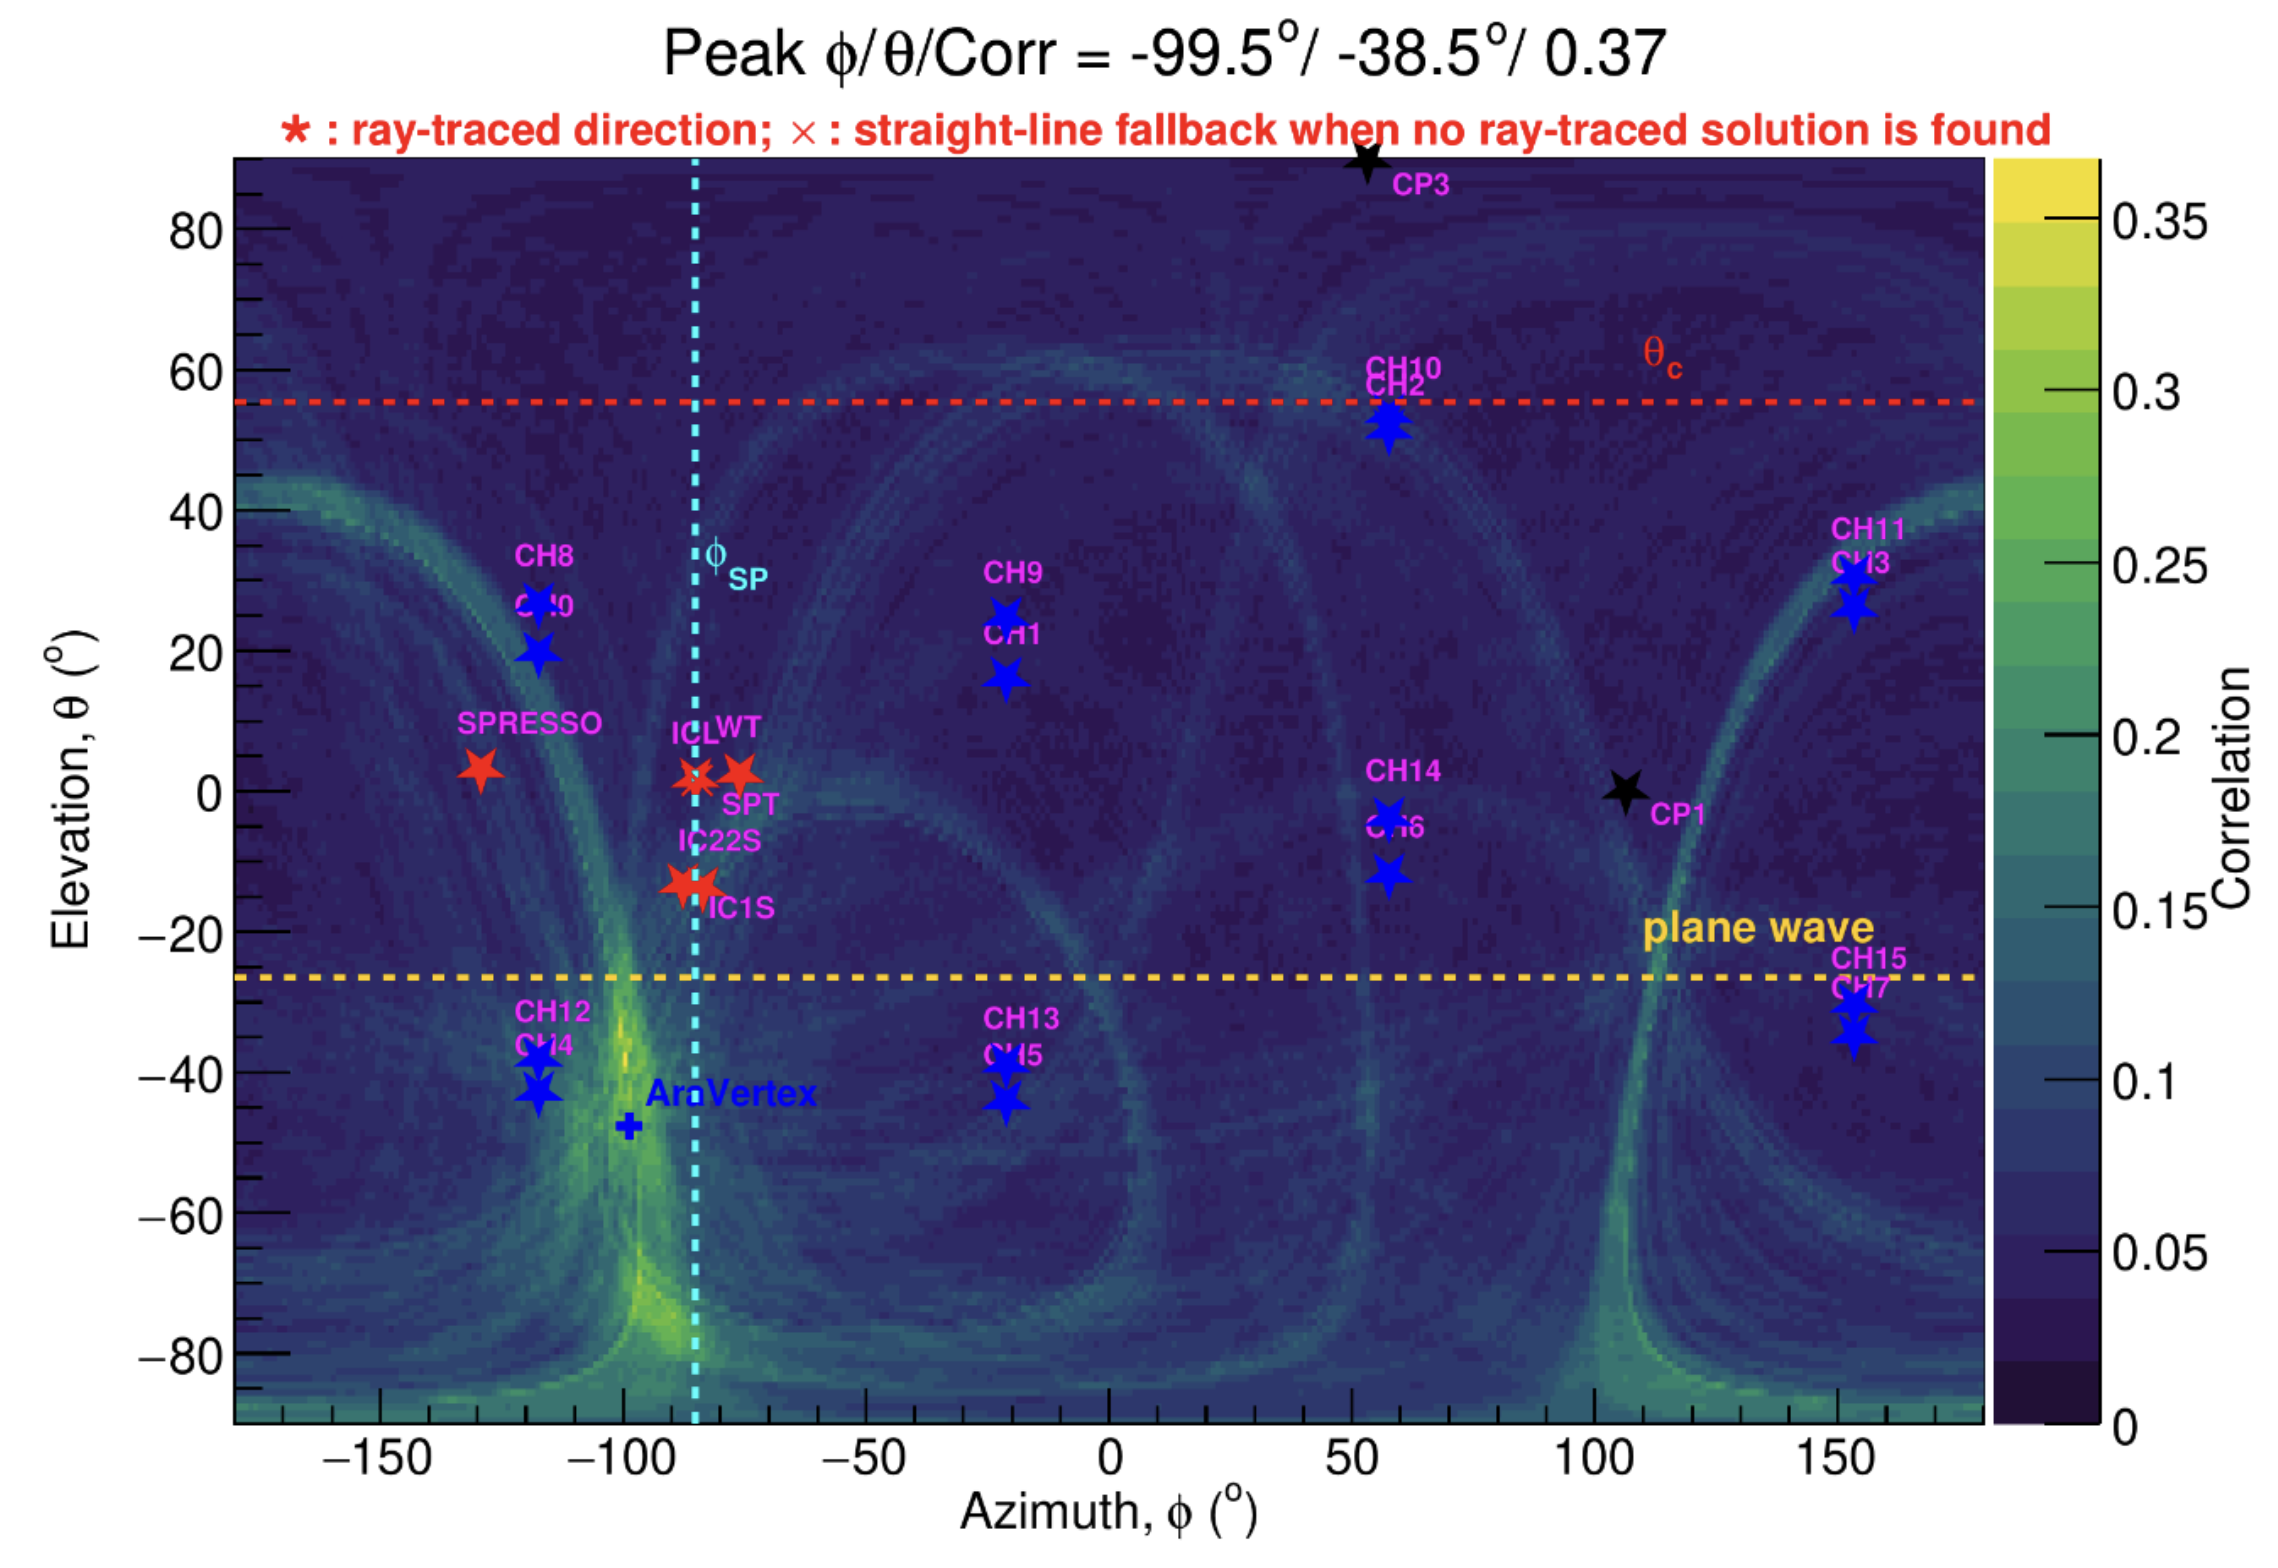
\includegraphics[
          width=\linewidth,
          alt={}
        ]{sections/5sa-analysis/images/passingevent_a5reco.png}
        \caption{
          Reconstruction of the A5 run 2899 event 64066, the event that occurred at the same time as the PA passing event. 
          The cross-correlation score assuming the signals originated from $-175.5^{\circ}\leq \phi \leq 175.5^{\circ}$ (x-axis) and $-89.5^{\circ}\leq \theta \leq 89.5^{\circ}$ (y-axis) are shown as a heat map.
          The location with the greatest correlation score is located at ($-99.5^{\circ}$, $-38.5^{\circ}$).
          The hit-time based reconstruction algorithm, \texttt{AraVertex}, reconstructs the event around ($-100^{\circ}$, $-48^{\circ}$) and is marked with a blue cross.
          Reconstruction assuming a plane wave solution estimates the signal originated from an elevation of $-26^{\circ}$ as is shown with the yellow, dashed line.
          All reconstructions suggest the event originates within $20^{\circ}$ in elevation (and azimuth for the interferometric and hit-time based reconstructions) of the A5 antennas 4 and 12 located around ($-120^{\circ}$, $-40^{\circ}$), marked with blue stars. 
        }
        \label{fig:passing_a5reco}
      \end{figure}

      Since the signals in the PA string and A5 strings 2, 3, and 4 resembled calibration pulsers but didn't reconstruct where we expect calibration pulses to come from, we added the locations of A5 and PA antennas to the reconstruction skymaps as shown in Fig~\ref{fig:passing_a5reco}.
      This showed that the AraVertex algorithm reconstructed the A5 event within $20^{\circ}$ of the locations of antennas 4 and 12. 
      The same effect was observed when we plotted the skymap of correlation scores for the A5 event's interferometric reconstruction using a map radius equal to the distance between A5 antenna 4 and the station center - the best interferometric reconstruction is $20^{\circ}$ away from the locations of antenna 4 and 12. 
      We repeated this exercise for the A4 event shown in Fig.~\ref{fig:a4outlier} and found the event reconstructed where antennas 6 and 14 are, the same channels exhibiting power surge behavior.
      The analysis presented in Ref.~\citep{ara_a23} also discovered 7 events of this nature which gave rise to the original Spark Event Cut.% \footnote{\url{https://aradocs.wipac.wisc.edu/cgi-bin/DocDB/ShowDocument?docid=2032}}.

      The impulsive signatures on the strings presented in Fig.~\ref{fig:a4outlier} were not understood when designing the Anomalous Channel Cut, but would not be classified as potential neutrino observations given the string of anomalous waveforms in the same event. 
      The anomalous waveforms were assumed to have been created by the data acquisition board which is housed in the vault at the surface, but as the impulsive signals in the same event resemble coherent radio emission reconstructing in deep ice, this suggests that the technical malfunction occurs on the string itself near the antennas. 
      This may be caused by the low noise amplifiers which are connected to and located next to each antenna, which can push power into the connected antenna, causing the antennas to temporally and spontaneously pulse radio waves like the calibration pulsers do.
      This may also be related to horizontally polarized antenna feeds, since no events like these occur after the 2019-2020 South Pole summer season.
      This was the season when all vertically polarized A5 antennas were connected to the PA data acquisition board and most horizontally polarized A5 antennas were left disconnected after the A5 board malfunctioned and stopped taking data (see Section~\ref{sec:pa_hardware} for more information).

      Based on these findings, an a posteriori cut was defined and applied to remove this class of technical backgrounds.
      We employ a cut that removes PA events within 0.05 seconds of A5 events that are cut by the Spark Event Cut defined in Section~\ref{sec:sec} or the Anomalous Channel Cut defined in Section~\ref{sec:acc}.
      219 A5 events were removed from the full sample by these cuts, leading to a negligible decrease in PA livetime of 21.9 seconds. 
      With the A1-A5 Anomalous Channel cut expanded to exclude nearby PA events, this event, which is clearly technical background, no longer passes all cuts and is rejected by this analysis.

      We have not found an explanation for why the A4 event occurred at the same time as the PA event which passed the analysis (and the corresponding A5 event).
      Over the whole array and livetime, the number of events removed by the Spark Event and Anomalous Channel cut is 13 for A1, 150 for A2, 90 for A3, 202 for A4, and 219 for A5. 
      Of these events, there were at most 3 coincident events across stations so we expect the simultaneous A4 and A5+PA spark events was a rare occurrence, though we have not completely ruled out that the A4 and A5 events were not random.
      User login records for the South Pole remote access computer for April 4, 2018 indicate there was an active user at the time of the PA passing event, but they were not affiliated with ARA, so it is unlikely that the events were associated with this person.
  
\section{Results\label{sec:5sa_results}}

    In absence of an observed neutrino event, we construct an upper limit on the observed neutrino flux.
    The 90\% confidence level upper limit factor relies on the number of observed events (0, for this analysis) and the number of expected backgrounds. 
    We modeled backgrounds for the Geometry Cut, the Zenith Cut, and the LDA Cut.
    As discussed in Section~\ref{sec:gc}, the windows used in the Geometry Cut were defined such that the number of passing events was $2\times10^{-5}$ for the 10\% sample, meaning $2\times10^{-4}$ for the 100\% sample. 
    We multiply this by our expected untagged calibration pulser event rate of $10^{-4}$ for each station to achieve a background leakage of $2\times 10^{-8}$ events per window.  
    For both the Zenith Cut and LDA Cut, the number of expected background events is an output from the optimization performed in Section~\ref{sec:optimization}. 
    The number of background events per station and array-wide are presented in Table~\ref{tab:backgrounds}.

    \begin{figure}
      \centering
      \includegraphics[
        width=\linewidth,
        alt={}
      ]{sections/5sa-analysis/images/Background-Leakage.pdf}
      \caption{
        The number of background events expected (based on the fits to 10\% of the data) to ``leak'' into the final dataset based on the Geometry Cut and models defined in Section~\ref{sec:gc}, the Zenith Cut defined in Section~\ref{sec:zc_slc} and Optimized in Section~\ref{sec:optimization}, and the thermal-like LDA cut defined in Section~\ref{sec:lda} and optimized in Section~\ref{sec:optimization}.
        The number of leaked events is presented per station and for the array as a whole.
      }
      \label{tab:backgrounds}
    \end{figure}

    The final upper limit of this analysis is established using the simulations defined in Chapter~\ref{chap:veff} and Eq.~\ref{eq:phi_UL} and is reported in Tab~\ref{tab:results}.

    \begin{table}[ht!]
      \centering
      \begin{tabular}{|c|c|}
        \hline
        & $N_{\text{events}}$ \\
        \hline
        Background & 0.13 \\
        Observed & 0 \\
        90\% CL Upper Limit & 2.44 \\
        \hline
      \end{tabular}
      \caption{
        Expected number of background events, observed number of events that passed this analysis, and the \citep{feldman_cousins} 90\% confidence level upper limit on the number of events for this analysis.
      }
      \label{tab:results}
    \end{table}

    The differential upper limit to the cosmic neutrino flux is shown as the bold line in Fig.~\ref{fig:5sa_sensitivity}, with the analysis' Single Event Sensitivity (SES) and trigger level upper limit. 
    % We establish 90\% confidence when stating that the true rate of neutrinos in each energy bin could be up to 2.44, according to the Feldman Cousins formulation.
    The SES represents the flux required to observe at least 1 event in each energy bin.
    The number of events we predict exist in our sample after all cuts have been applied is given in Tab.~\ref{tab:5sa_eventrates}.
    The sensitivity achieved by this analysis can be compared to results by other experiments and a collection of neutrino flux models, including the models that yield the greatest neutrino flux from \citep{flux-kotera,flux-muzio,flux-ahlers-halzen}.

    \begin{figure}
        \centering
        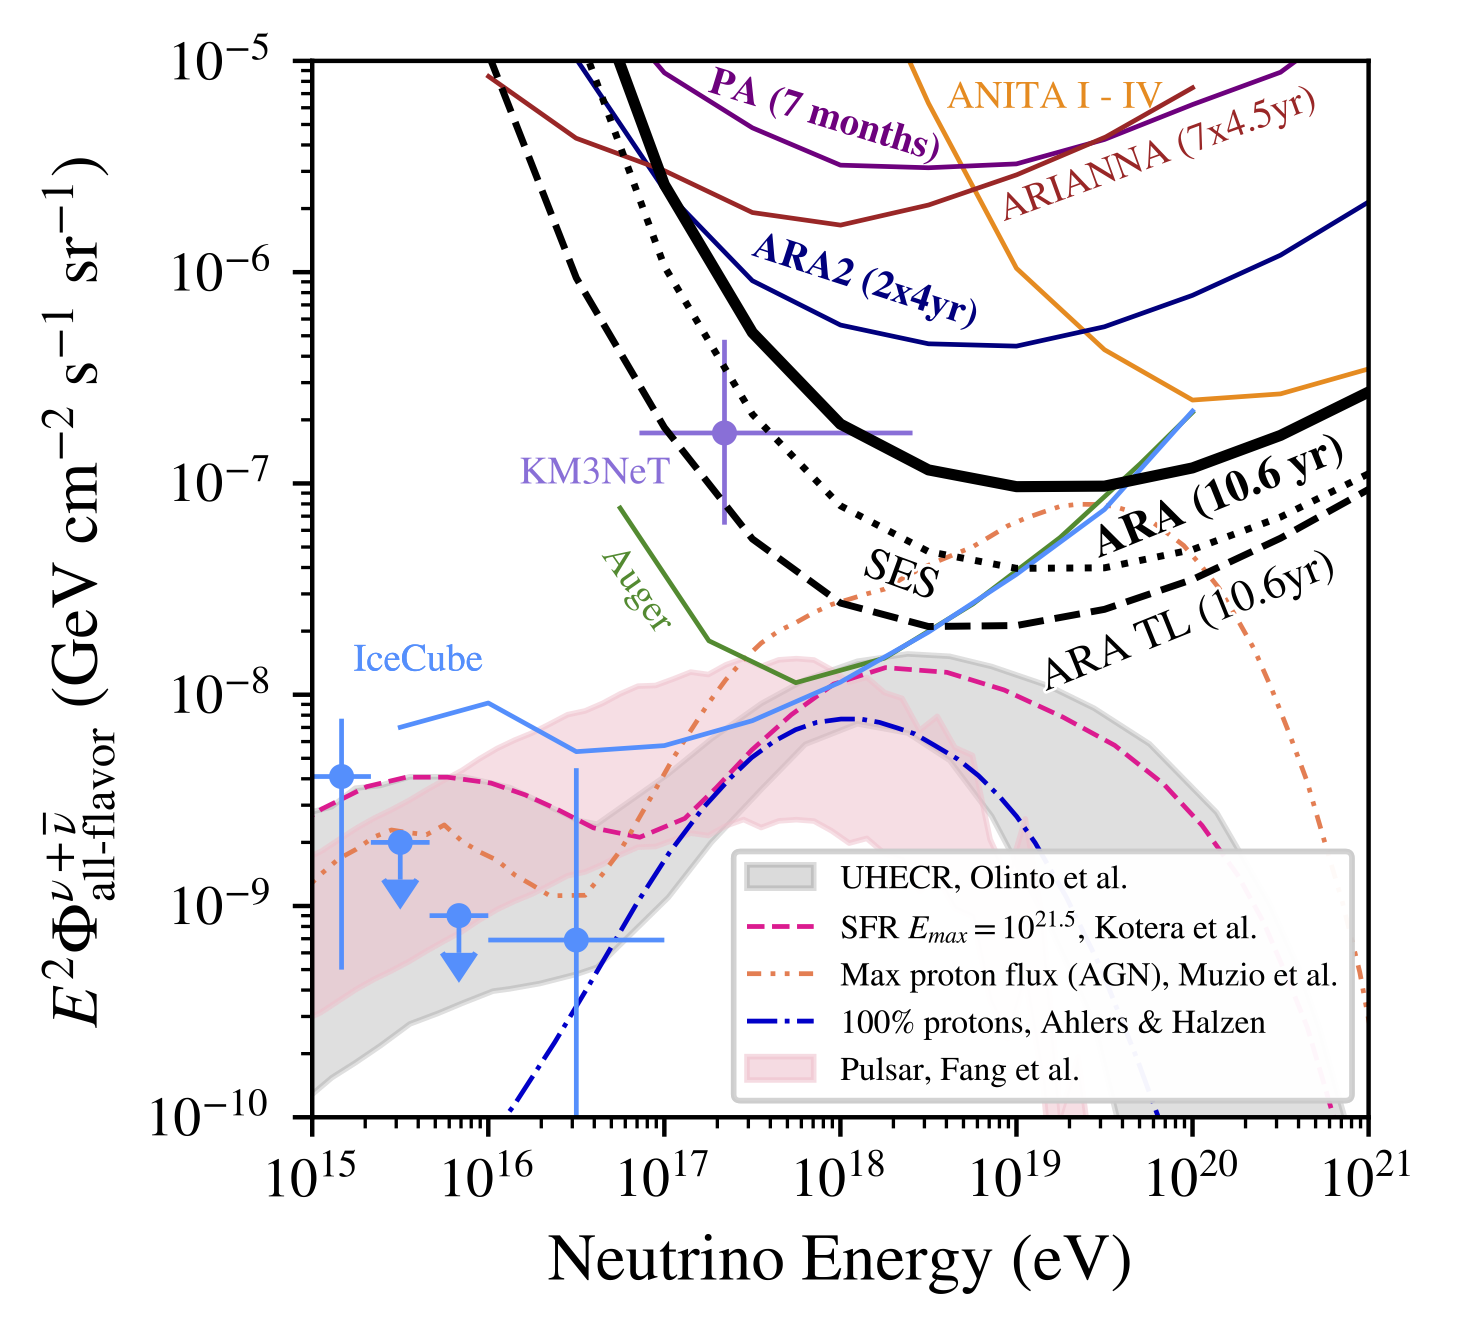
\includegraphics[
            width=0.75\textwidth,
            alt={}
        ]{sections/5sa-analysis/images/5sa_e2Sensitivity_astrocosmo-5SA.pdf}
        \caption{
          Analysis level sensitivity of the array-wide neutrino search through 10.6 years of ARA data (solid black curve). 
          The single event sensitivity (SES) of the analysis level sensitivity is also presented (dotted black curve) along with the trigger level sensitivity (ARA TL, dashed black curve).
          Previous experimental results from IceCube~\citep{icecube_search-ehe, icecube_search-combined-fit}, KM3NeT~\citep{km3net_neutrino}, Auger~\citep{flux-auger}, ARIANNA~\citep{arianna_testbed}, ANITA I--IV~\citep{anita_iv}, and earlier ARA analyses (ARA2~\citep{ara_a23} and PA~\citep{ara_pa_analysis}) are also shown (colored solid).
          A selection of optimistic cosmogenic and astrophysical neutrino flux models are presented as well~\citep{flux-kotera,flux-muzio,flux-ahlers-halzen,flux-fang-pulsars, flux_olinto}.
        }
        \label{fig:5sa_sensitivity}
    \end{figure}

    \begin{table}
      \centering
      \begin{tabular}{ 
          >{\centering\arraybackslash}m{5cm} 
          >{\centering\arraybackslash}m{3cm} | 
          >{\centering\arraybackslash}m{3cm} 
          >{\centering\arraybackslash}m{3cm} 
        }
        Model & Model Type & $N_{\text{events}}$ \hspace{0.5cm} (Trigger Level) & $N_{\text{events}}$ \hspace{0.5cm}  (Analysis Level) \\
        \hline
        \hline
        Global Upper Limit \citep{icecube_search-ehe, anita_iv} & Experimental & 21.64 & 6.24 \\
        \citep{flux-muzio} & Cosmogenic & 12.11 & 2.79 \\
        \citep{flux-kotera} & Cosmogenic & 2.09 & 0.41 \\
        100\% Protons \citep{flux-ahlers-halzen} & Cosmogenic & 0.87 & 0.15 \\
        \citep{flux-fang-pulsars} & Astrophysical & 1.31 & 0.20 \\
        \citep{km3net_neutrino} & Experiment & 12.30 & 1.73 \\
        \citep{icecube_search_extension} & Experiment & 0.19 & 0.03 \\
      \end{tabular}
      \caption{
        Expected number of neutrino events expected at trigger level and at analysis level based on various astrophysical models, cosmogenic models, and experimental fluxes and upper limits. 
        These results may be compared to the Feldman-Cousins upper limit of 2.44 events, established by the observation of 0 events on an expected background of 0.13 events in this analysis.
      }
      \label{tab:5sa_eventrates}
    \end{table}